\section{Pendahuluan}
\subsection{Latar Belakang}
Digital filter adalah suatu alat yang digunakan untuk memodifikasi sinyal digital dengan cara menghilangkan atau mengurangi noise, menghilangkan komponen frekuensi tertentu, dan memperbaiki kualitas sinyal. 
Digital filter sangat penting dalam berbagai aplikasi, seperti pengolahan sinyal audio, pengukuran, dan sistem monitoring.
\\\\
Ada dua jenis utama digital filter: Filter Infinite Impulse Response (IIR) dan Filter Finite Impulse Response (FIR).
Filter IIR: Menggunakan konsep feedback dan feed forward untuk menghasilkan output yang berdasarkan input sekarang, input sebelumnya, dan output sebelumnya. Filter IIR dapat memiliki respon frekuensi yang lebih kompleks dan dapat digunakan untuk aplikasi yang memerlukan pengurangan noise yang lebih efektif.
Filter FIR: Menggunakan koefisien yang ditetapkan secara eksplisit untuk menghasilkan output yang berdasarkan input sekarang saja. Filter FIR memiliki respon frekuensi yang lebih sederhana dan lebih mudah untuk dirancang, tetapi dapat lebih efektif dalam menghilangkan noise yang memiliki frekuensi tertentu.
\\\\
Dalam sistem monitoring, digital filter digunakan untuk menghilangkan noise dan memperbaiki kualitas data sensor. 
Misalnya, dalam pengukuran suhu, digital filter digunakan untuk menghilangkan noise yang dapat mempengaruhi akurasi pengukuran suhu. 

\subsection{Maksud dan Tujuan}
Memahami konsep dan aplikasi digital filter pada pengolahan sinyal digital.
\subsection{Hasil yang diharapkan}
Memahami hasil sinyal sebelum dan sesudah dilakukan digital filter.

%===========================================================%
\section{Tugas Pendahuluan}
\begin{center}
	\colorbox{cyan!30}{\parbox{0.8\linewidth}{
    \begin{enumerate}
        \item Apa itu PPTP dan bagaimana cara kerjanya?
        \item Apa kelebihan dan kekurangan dari penggunaan PPTP dibandingkan protokol VPN lainnya seperti L2TP atau OpenVPN?
    \end{enumerate}}}
\end{center}

%===========================================================%
\section{Alat dan Bahan}
\begin{itemize}[label=$\bullet$, itemsep=-1pt, leftmargin=*]
	\item 2 buah Cloud Core Router
	\item 3 Kabel UTP (LAN)
	\item 2 buah Laptop
	\item Software Winbox
\end{itemize}

%===========================================================%
\section{Jangka Waktu Pelaksanaan}
Pemahaman dan konfigurasi 1 jam.

%===========================================================%
\section{Penjelasan dan Tahapan Konfigurasi}

%======================PERCOBAAN 1==========================%
\begin{center}
    \textbf{Konfigurasi PC 1}
    \begin{enumerate}
        \item Buka aplikasi Winbox pada PC dan lakukan hubungkan ke Router. Pastikan Login terisi “admin”, Klik Neighbors > Klik Refresh > Pilih Router yang ingin disambungkan > Klik Connect.
        \begin{figure}[H]
			\centering
			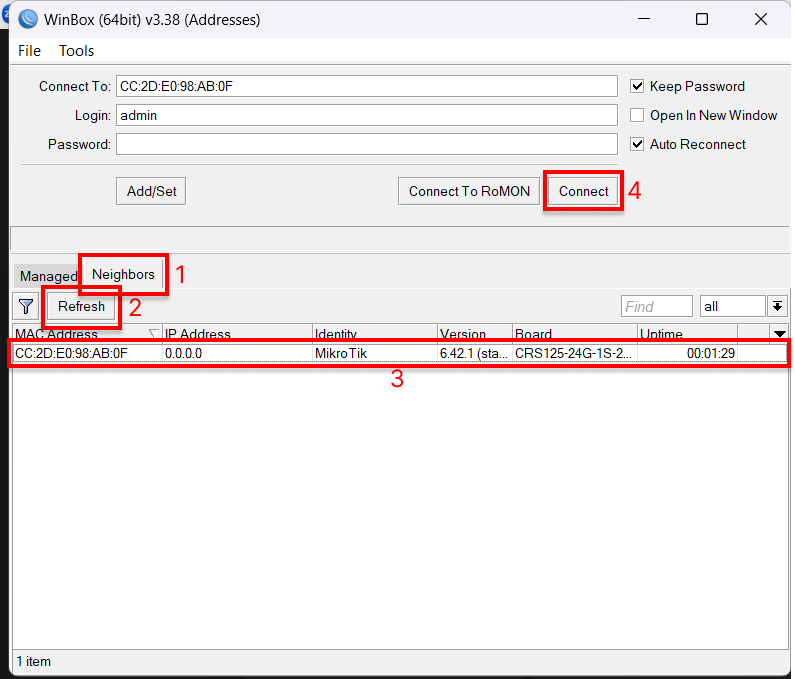
\includegraphics[width=0.5\linewidth]{P4/img/pc1/Step 1.png}
			\caption{Step 1}
			\label{fig:Step 1(PC 1)}
		\end{figure}
        \item Jadikan Router menjadi DHCP Client agar bisa mendapat IP address dari Internet ITS. IP > Klik DHCP Client > Tambahkan DHCP Client > Pilih interface yang terhubung dengan Internet (ether2)> Klik Apply > Klik OK. Kita bisa memastikan koneksi ke internet dengan cara melakukan tes ping ke alamat IP 8.8.8.8
        \begin{figure}[H]
			\centering
			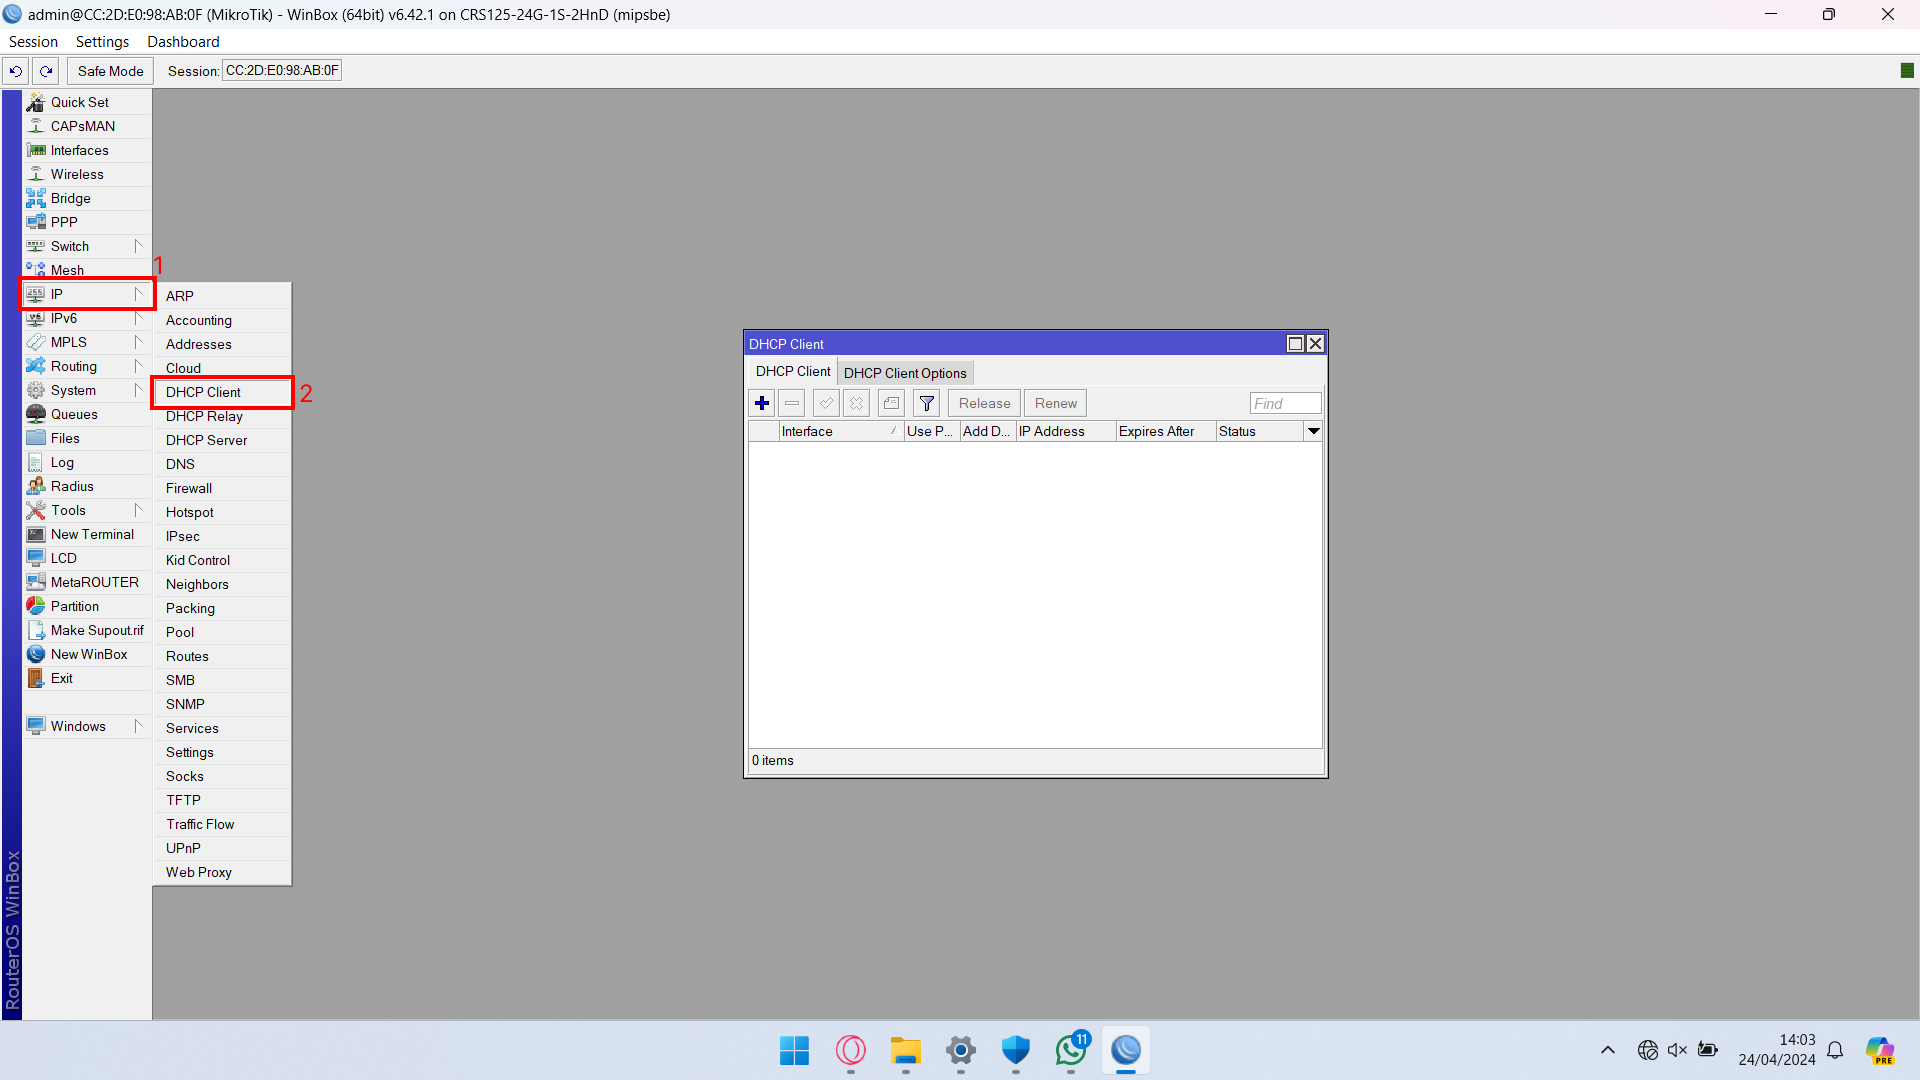
\includegraphics[width=0.5\linewidth]{P4/img/pc1/Step 2.1.png}
			\caption{Step 2.1}
			\label{fig:Step 2.1(PC 1)}
        \end{figure}
        \begin{figure}[H]
			\centering
			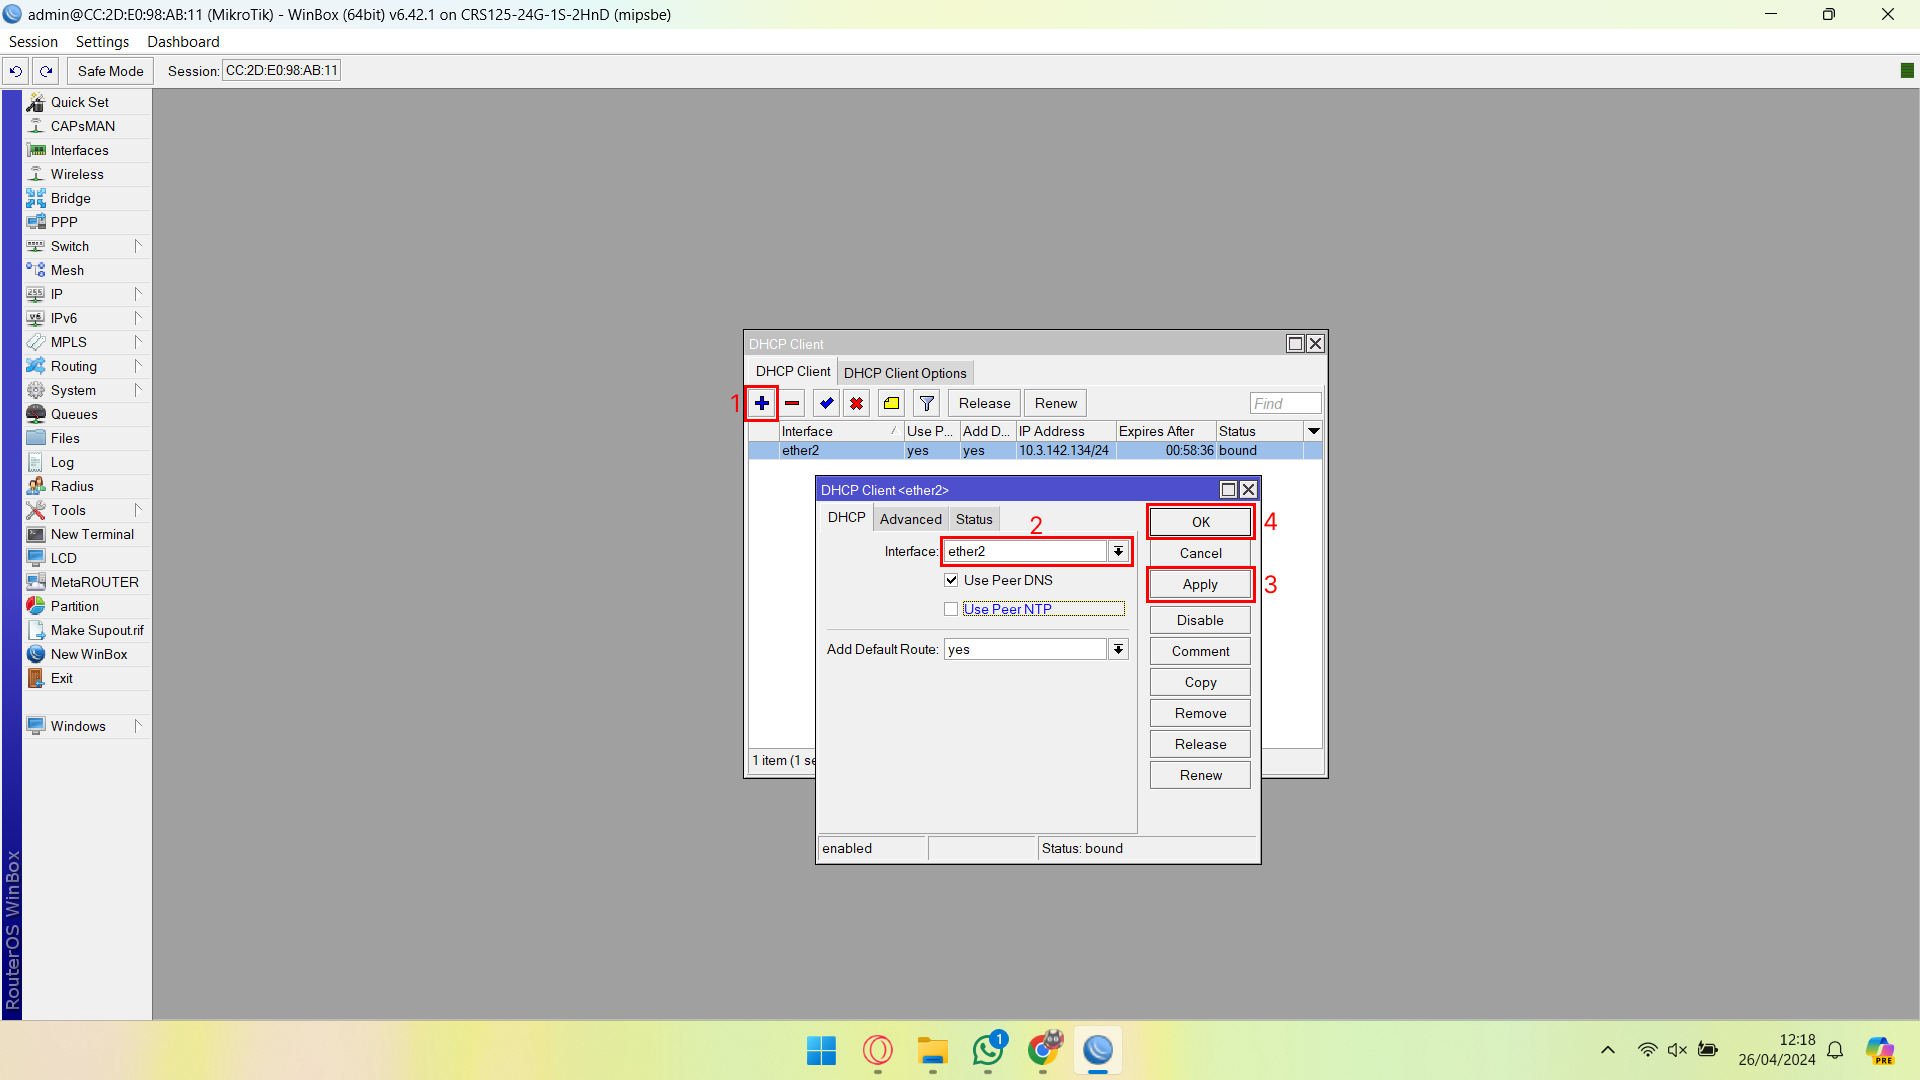
\includegraphics[width=0.8\linewidth]{P4/img/pc1/Step 2.2.png}
			\caption{Step 2.2}
			\label{fig:Step 2.2(PC 1)}
		\end{figure}
        \item Buat IP address baru pada Router 1 untuk menghubungkan PC 1 dengan Router 1. Tambahkan IP address > Isi address > Pilih Interface yang terhubung ke PC (ether4) > Klik Apply > Klik OK.
        \begin{figure}[H]
			\centering
			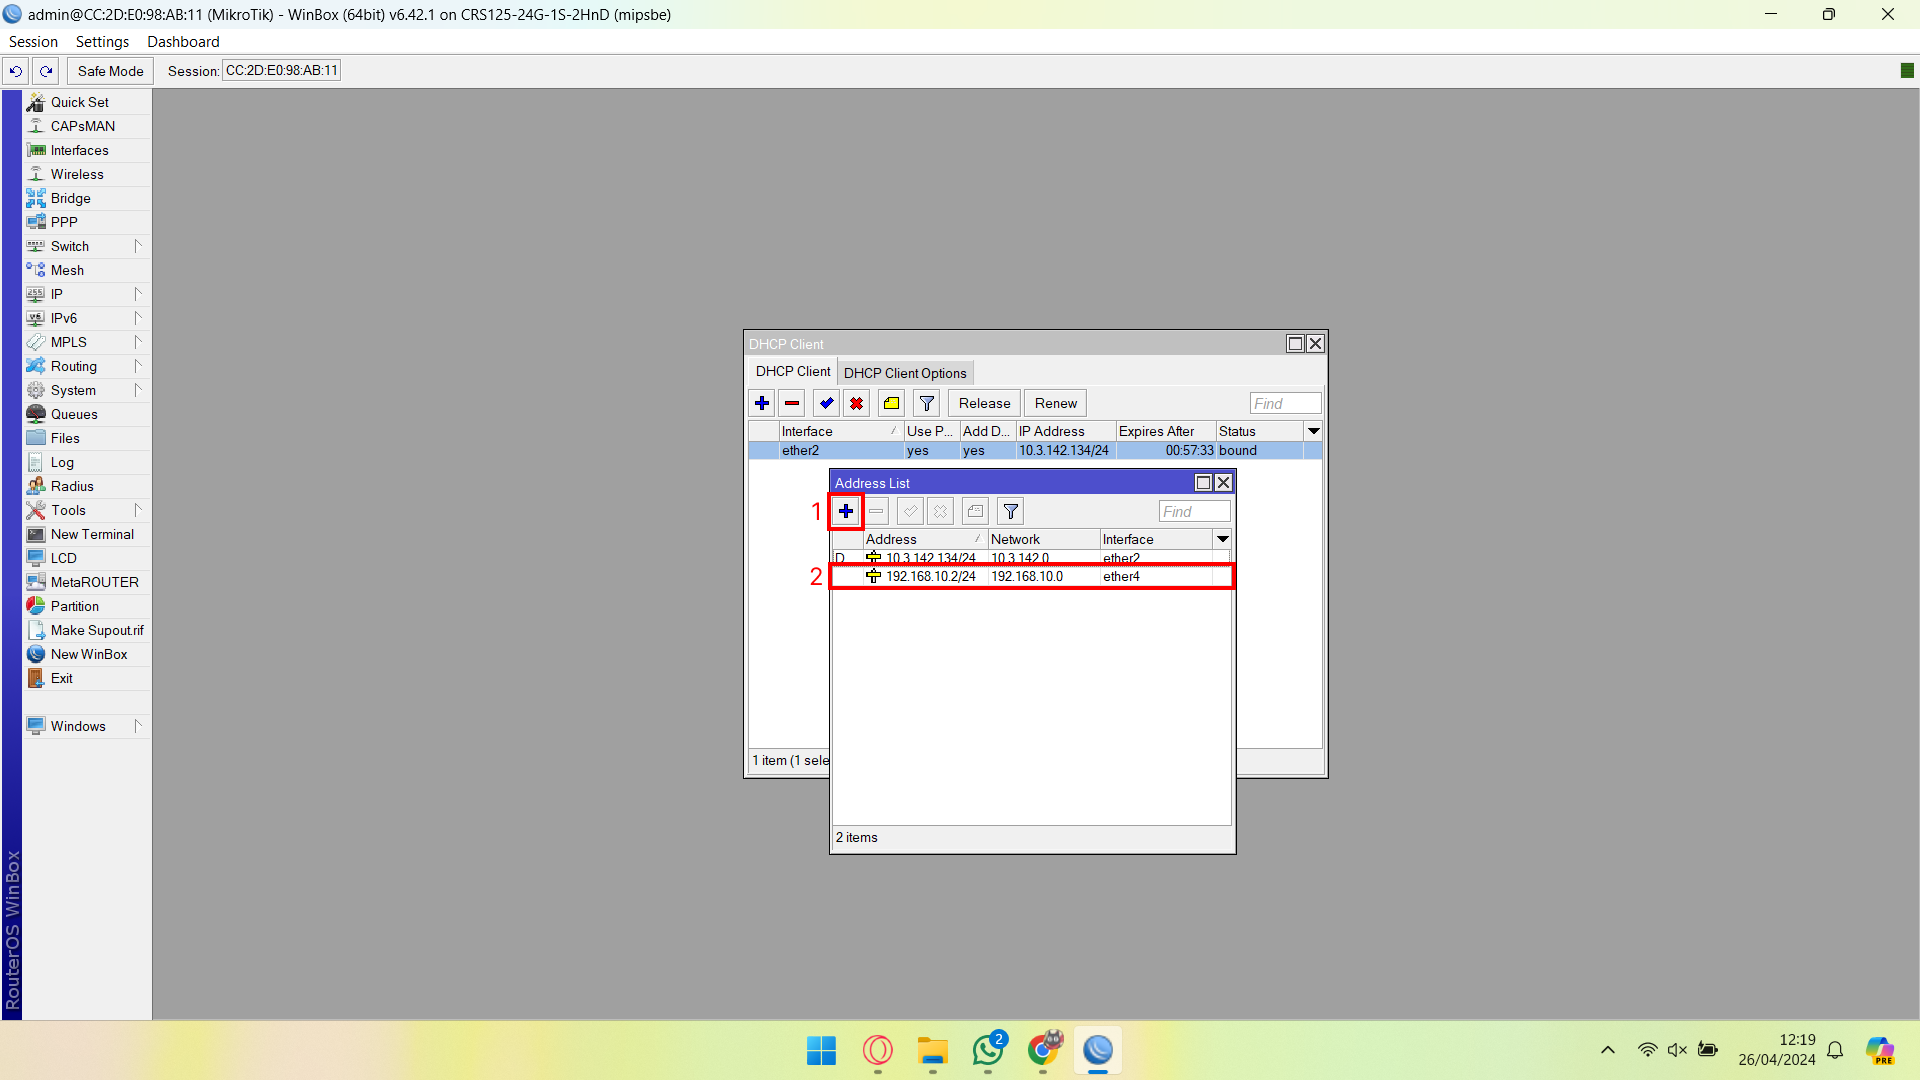
\includegraphics[width=0.8\linewidth]{P4/img/pc1/Step 3.png}
			\caption{Step 3}
			\label{fig:Step 3(PC 1)}
		\end{figure}
        \item Atur IP pada PC 1 dengan mengubah pengaturan pada setting ethernet. Ubah IP perangkat yang otomatis menjadi manual, pastikan IP PC 1 masih satu jaringan dengan IP lokal yang diinginkan, isi Gateway dengan IP address Router 1 yang tersambung dengan PC 1. Berikan IP address yang berbeda dengan contoh yang ada di modul.
        \begin{figure}[H]
			\centering
			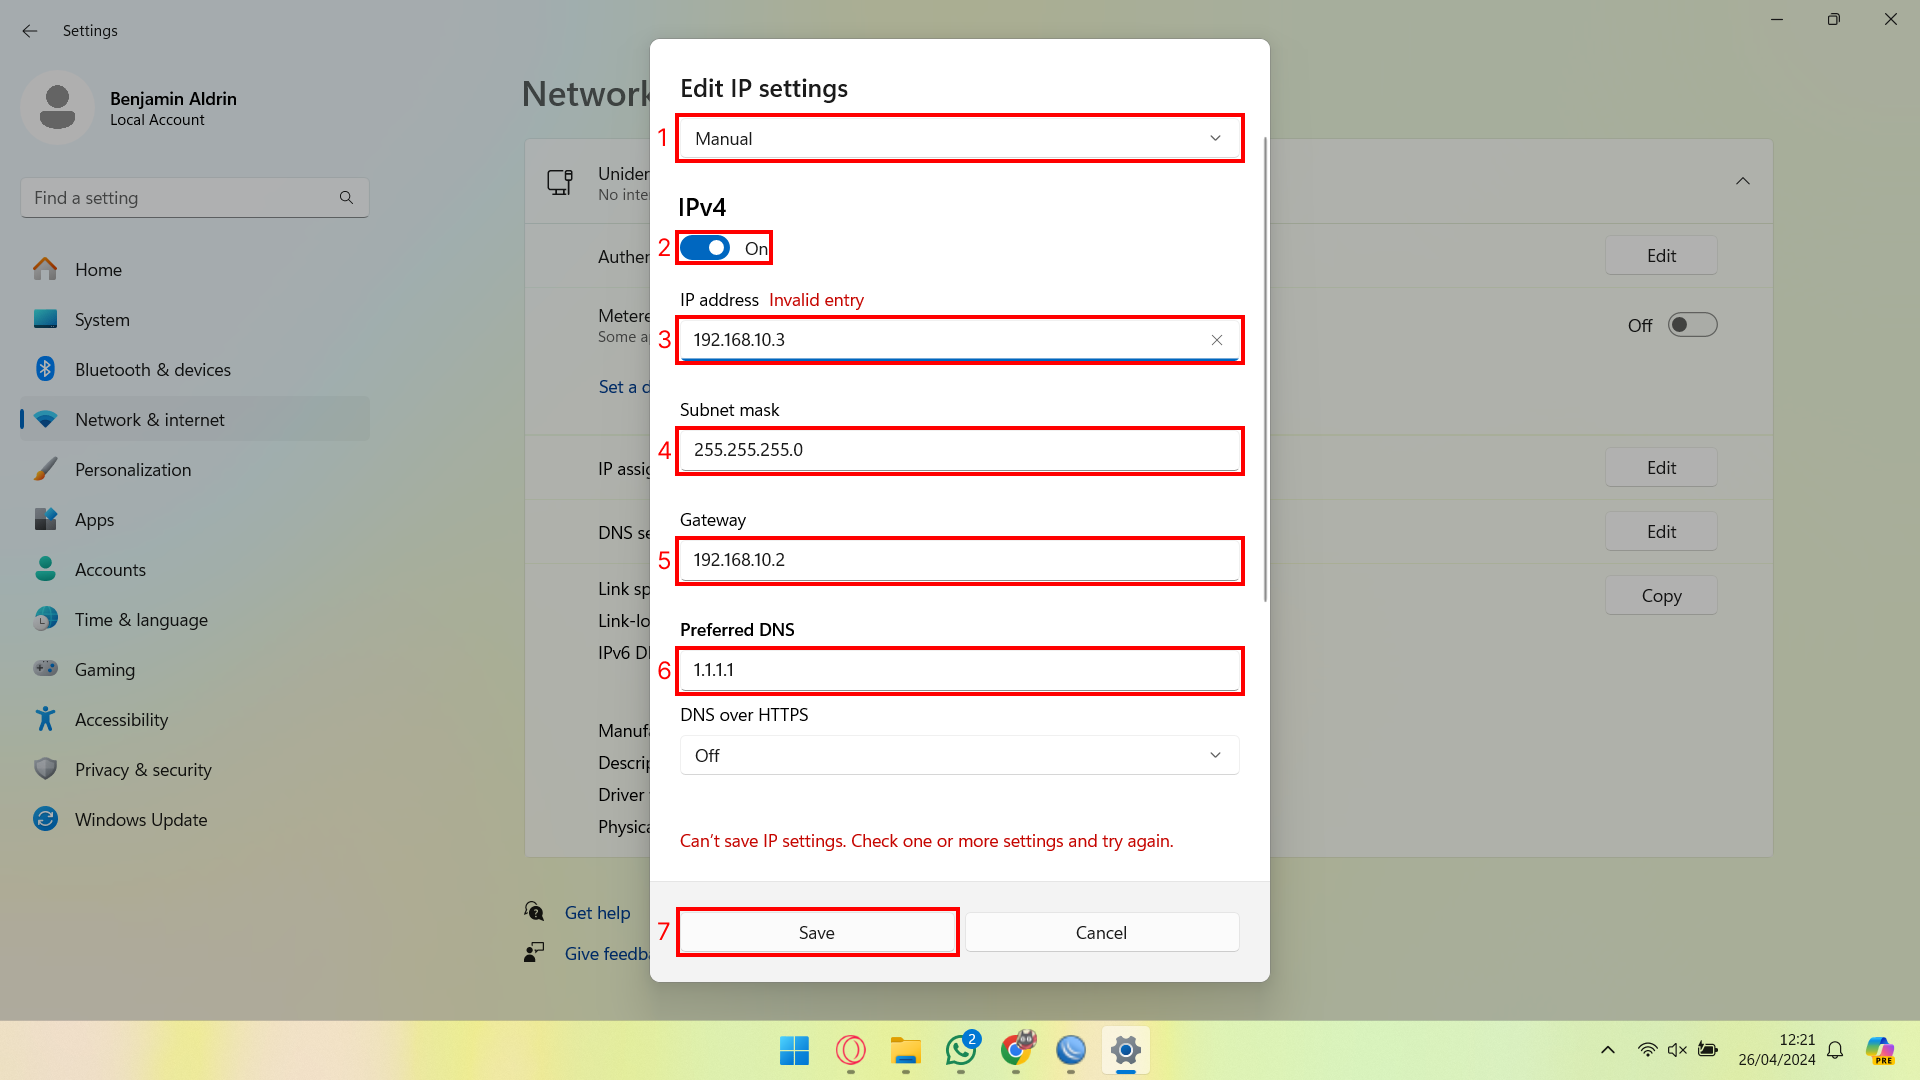
\includegraphics[width=0.8\linewidth]{P4/img/pc1/Step 4.png}
			\caption{Step 4}
			\label{fig:Step 4(PC 1)}
		\end{figure}
        \item Lakukan tes ping antara Router dengan PC1, untuk memastikan PC1 dan Router sudah terkoneksi.
        \begin{figure}[H]
			\centering
			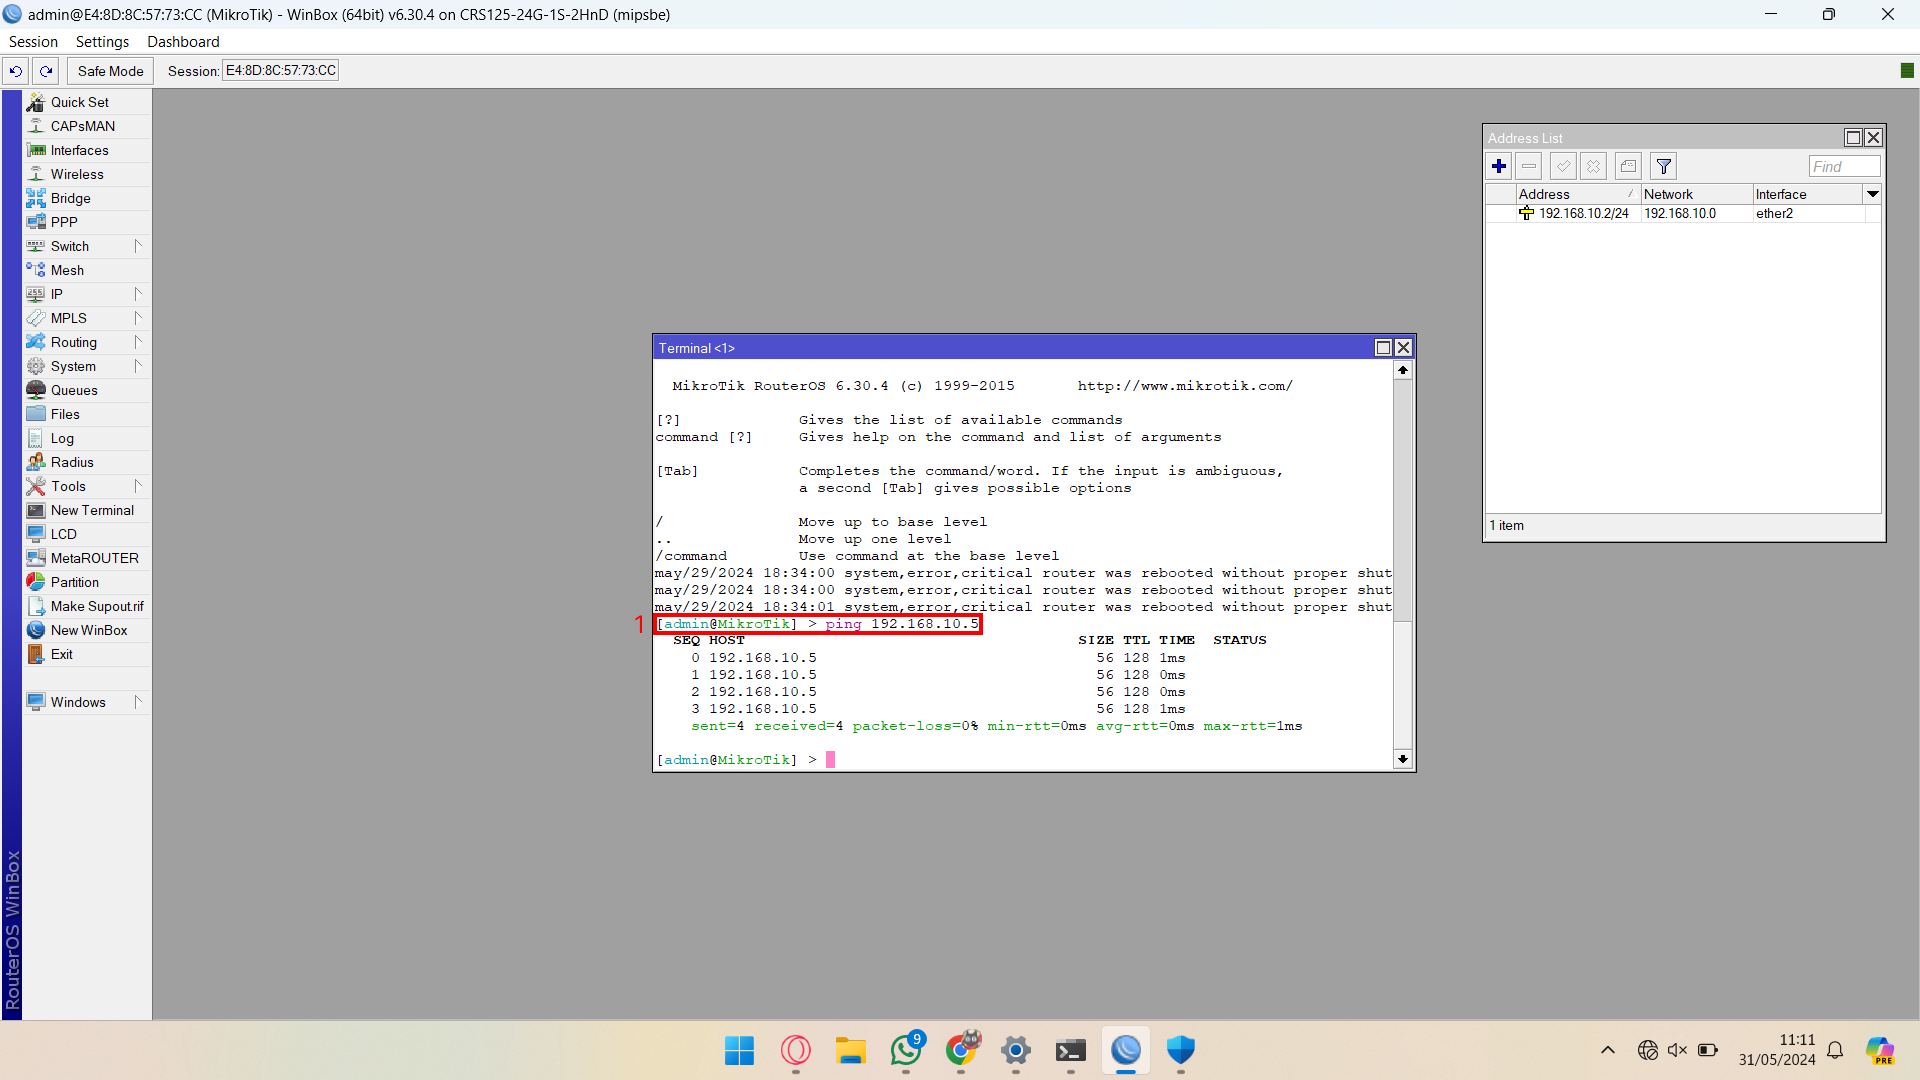
\includegraphics[width=0.8\linewidth]{P4/img/pc1/Step 5.png}
			\caption{Step 5}
			\label{fig:Step 5(PC 1)}
		\end{figure}
        \item Buat PPTP Server pada tab interface, dengan Default Profile “default -encryption”.
        \begin{figure}[H]
			\centering
			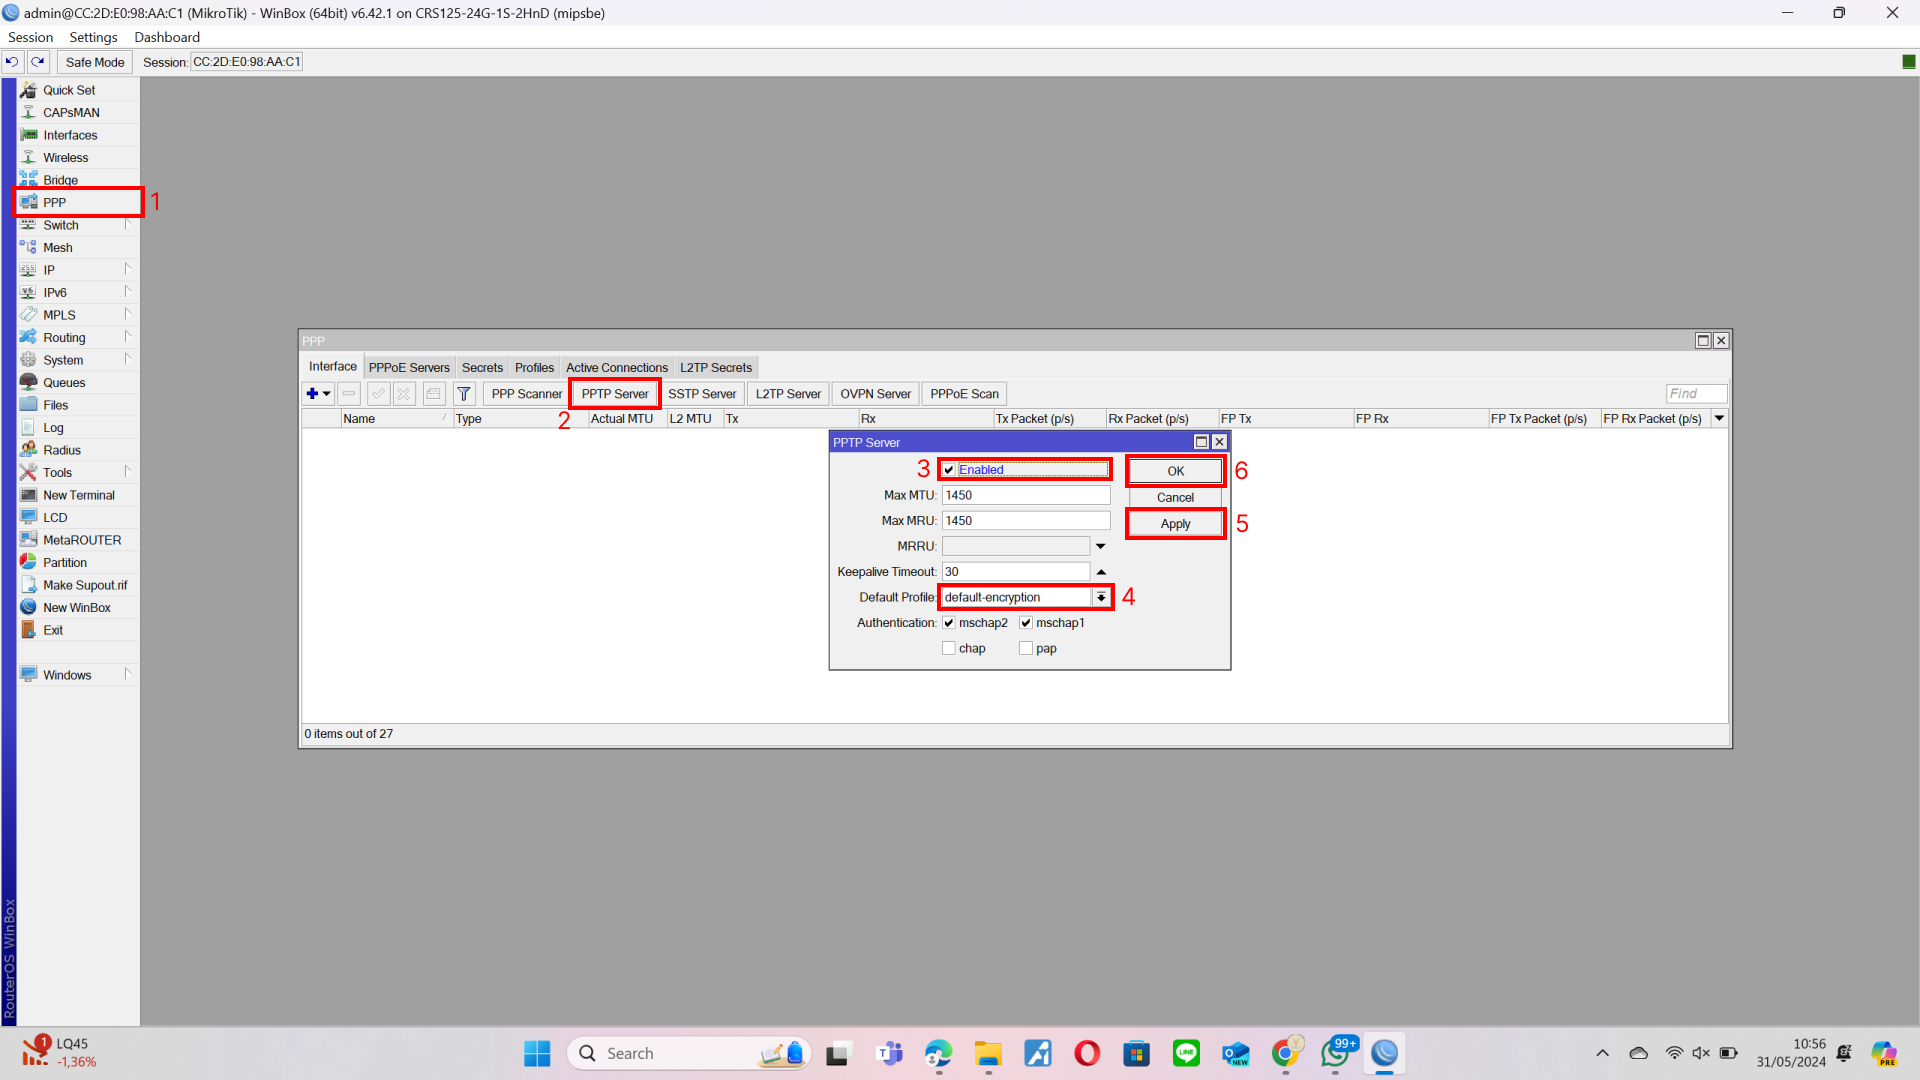
\includegraphics[width=0.8\linewidth]{P4/img/pc1/Step 6.png}
			\caption{Step 6}
			\label{fig:Step 6(PC 1)}
		\end{figure}
        \item Buat PPTP untuk client pada tab Secret, dengan konfigurasi Nama “PPTP”, Password “123456”, Service “pptp”, Profile “default”. Local Address adalah IP address tunnel pada sisi server, diisi dengan “10.10.10.2”. Remote Address adalah IP yang akan Client dapatkan, diisi dengan “10.10.10.3”. Pastikan Local Address dan Remote Address berada pada satu jaringan yang sama.
        \begin{figure}[H]
			\centering
			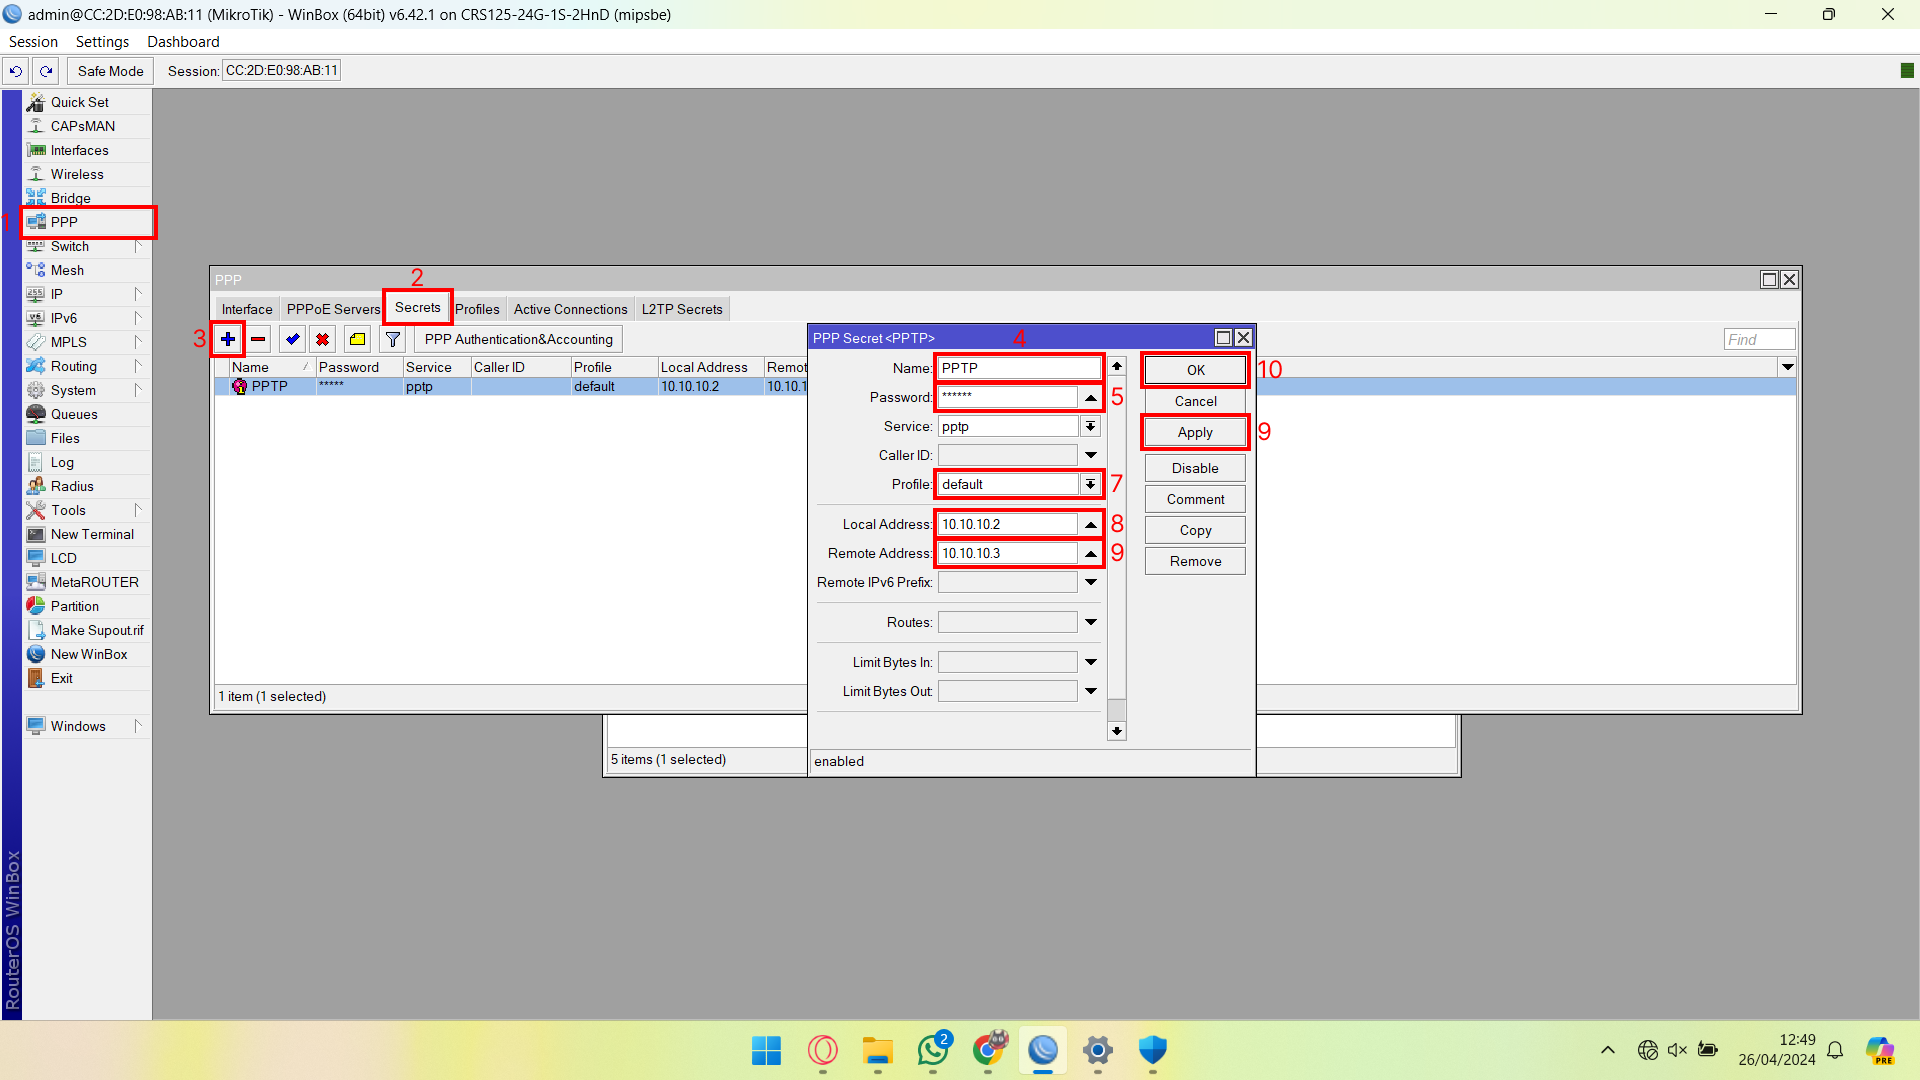
\includegraphics[width=0.8\linewidth]{P4/img/pc1/Step 7.png}
			\caption{Step 7}
			\label{fig:Step 7(PC 1)}
		\end{figure}
        \item Lakukan routing statis untuk menghubungkan PC1 dengan Internet. Buka pada tab IP > Routes, lalu tambahkan jaringan. Masukkan alamat jaringan yang ingin dituju, melalui alamat Gateway pada router 1
        \begin{figure}[H]
			\centering
			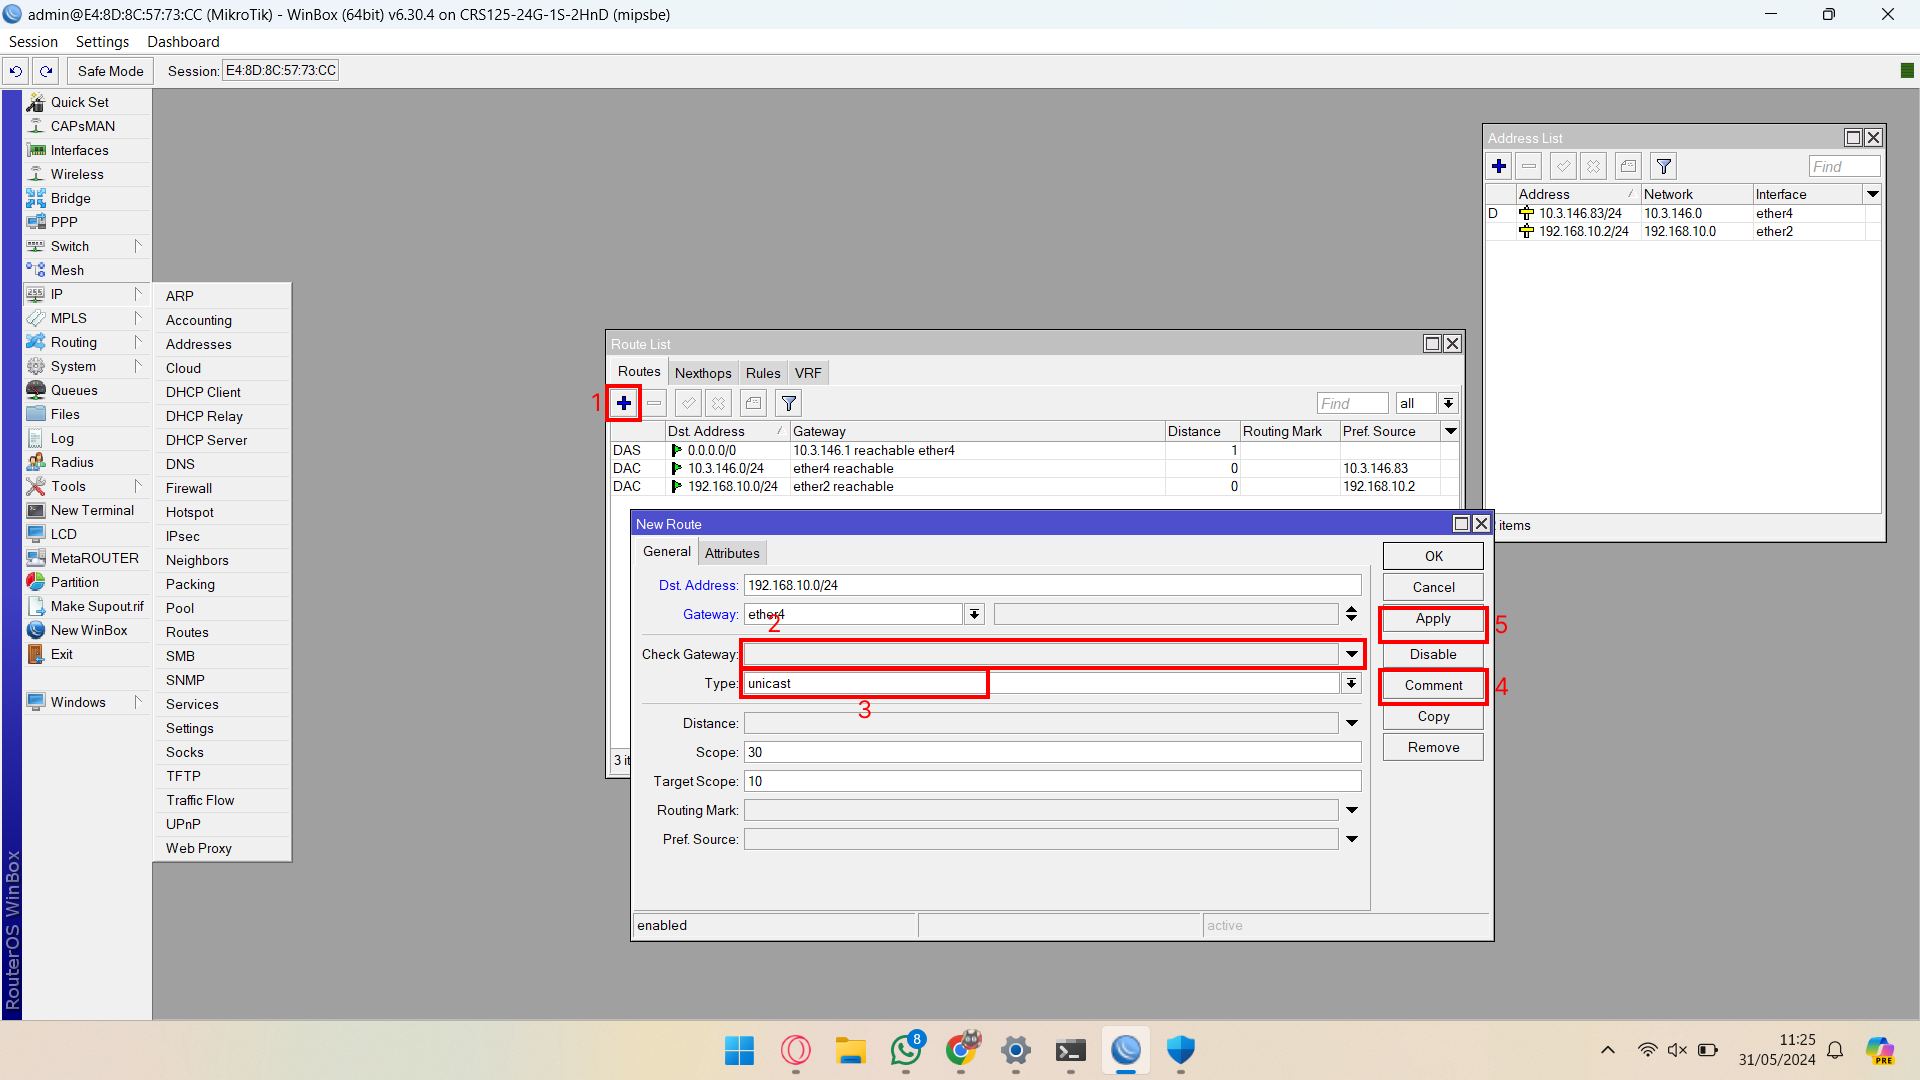
\includegraphics[width=0.8\linewidth]{P4/img/pc1/Step 8.png}
			\caption{Step 8}
			\label{fig:Step 8(PC 1)}
		\end{figure}
		\item Agar PC yang berada pada jaringan lokal dapat terhubung ke jaringan publik, dapat digunakan layanan NAT (Network Address Translation) yang akan menerjemahkan IP lokal beserta port perangkat agar dapat terhubung dengan jaringan publik. IP > Klik Firewall.
        \begin{figure}[H]
			\centering
			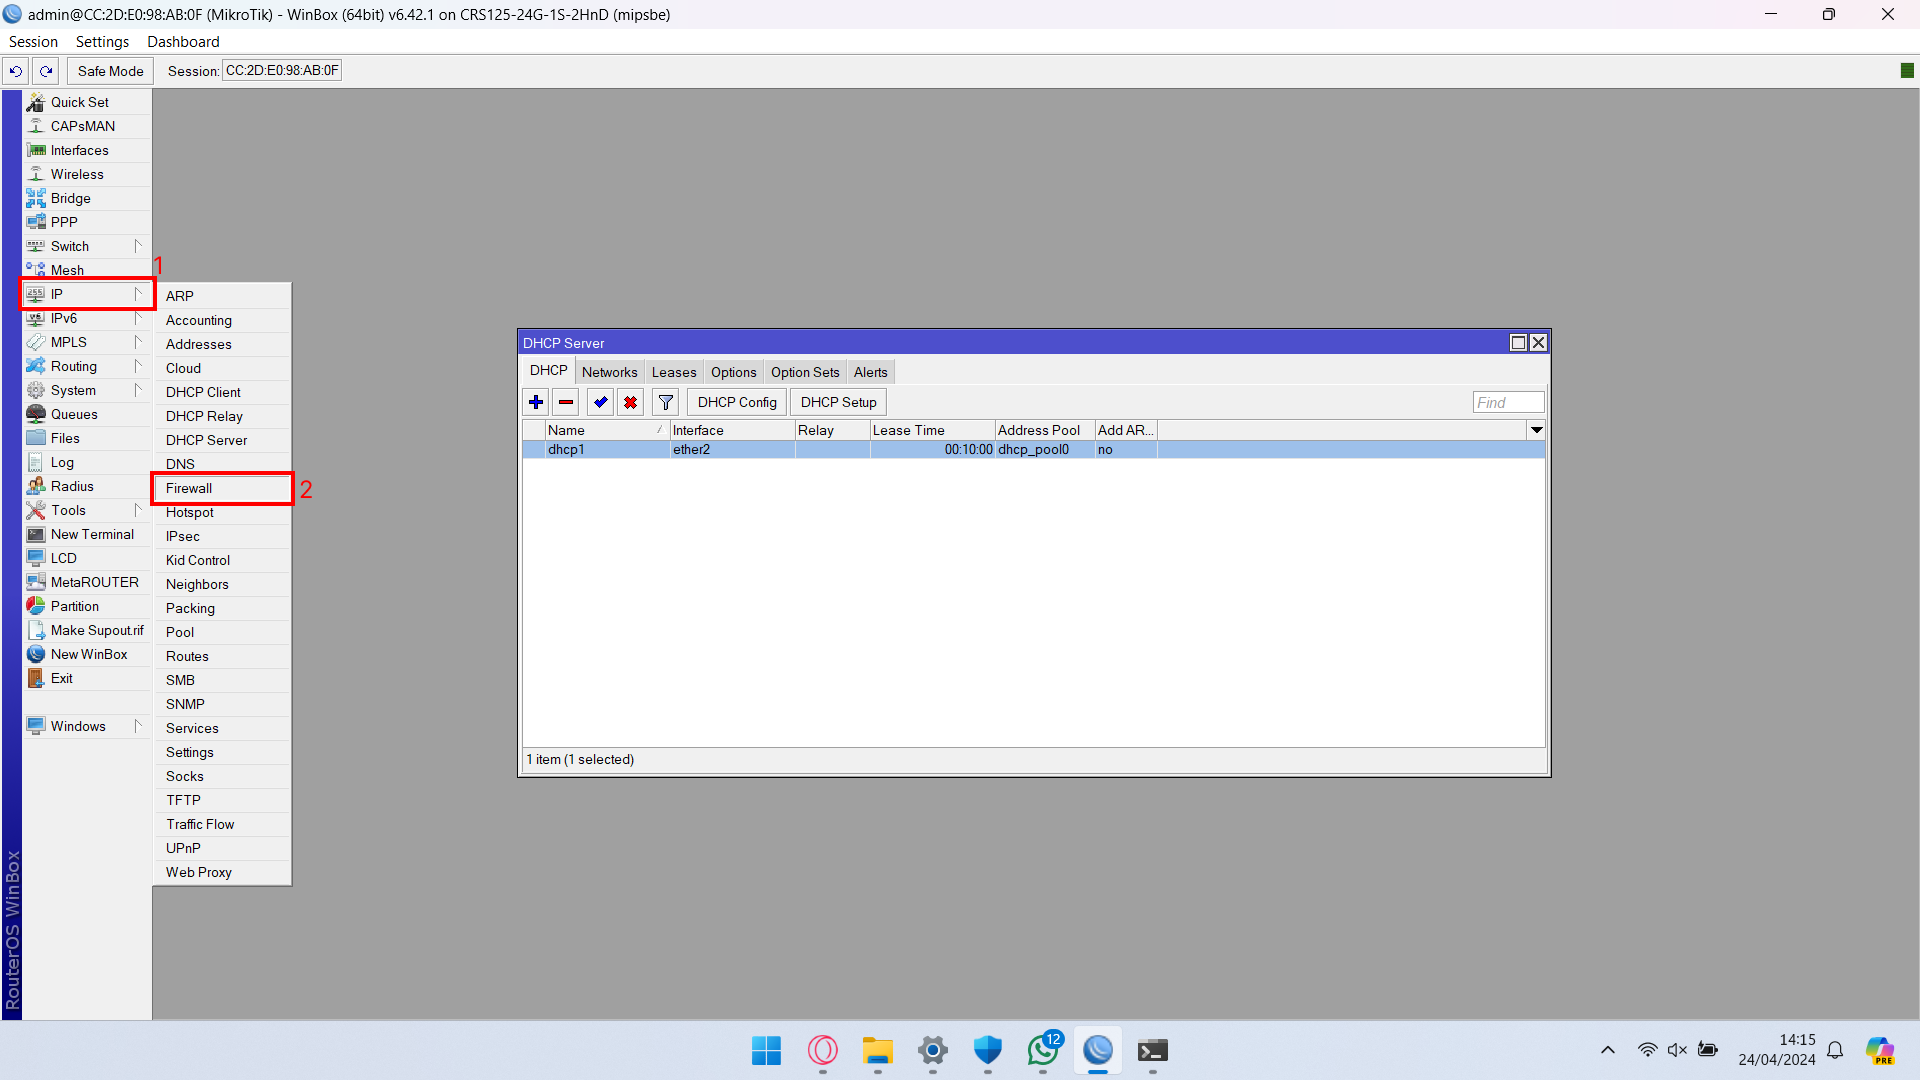
\includegraphics[width=0.8\linewidth]{P4/img/pc1/Step 16.png}
			\caption{Step 9}
			\label{fig:Step 9(PC 1)}
		\end{figure}
		\item Buat NAT baru. Klik tab NAT > Tambahkan NAT > Pada Opsi Chain pilih srcnat > Pilih Out Interface yaitu port pada Router yang terhubung dengan Internet(ether6) > Klik Apply. Tambahkan Action pada tab Action. Pada Opsi Action pilih masquerade > Klik Apply > Klik OK.
        \begin{figure}[H]
			\centering
			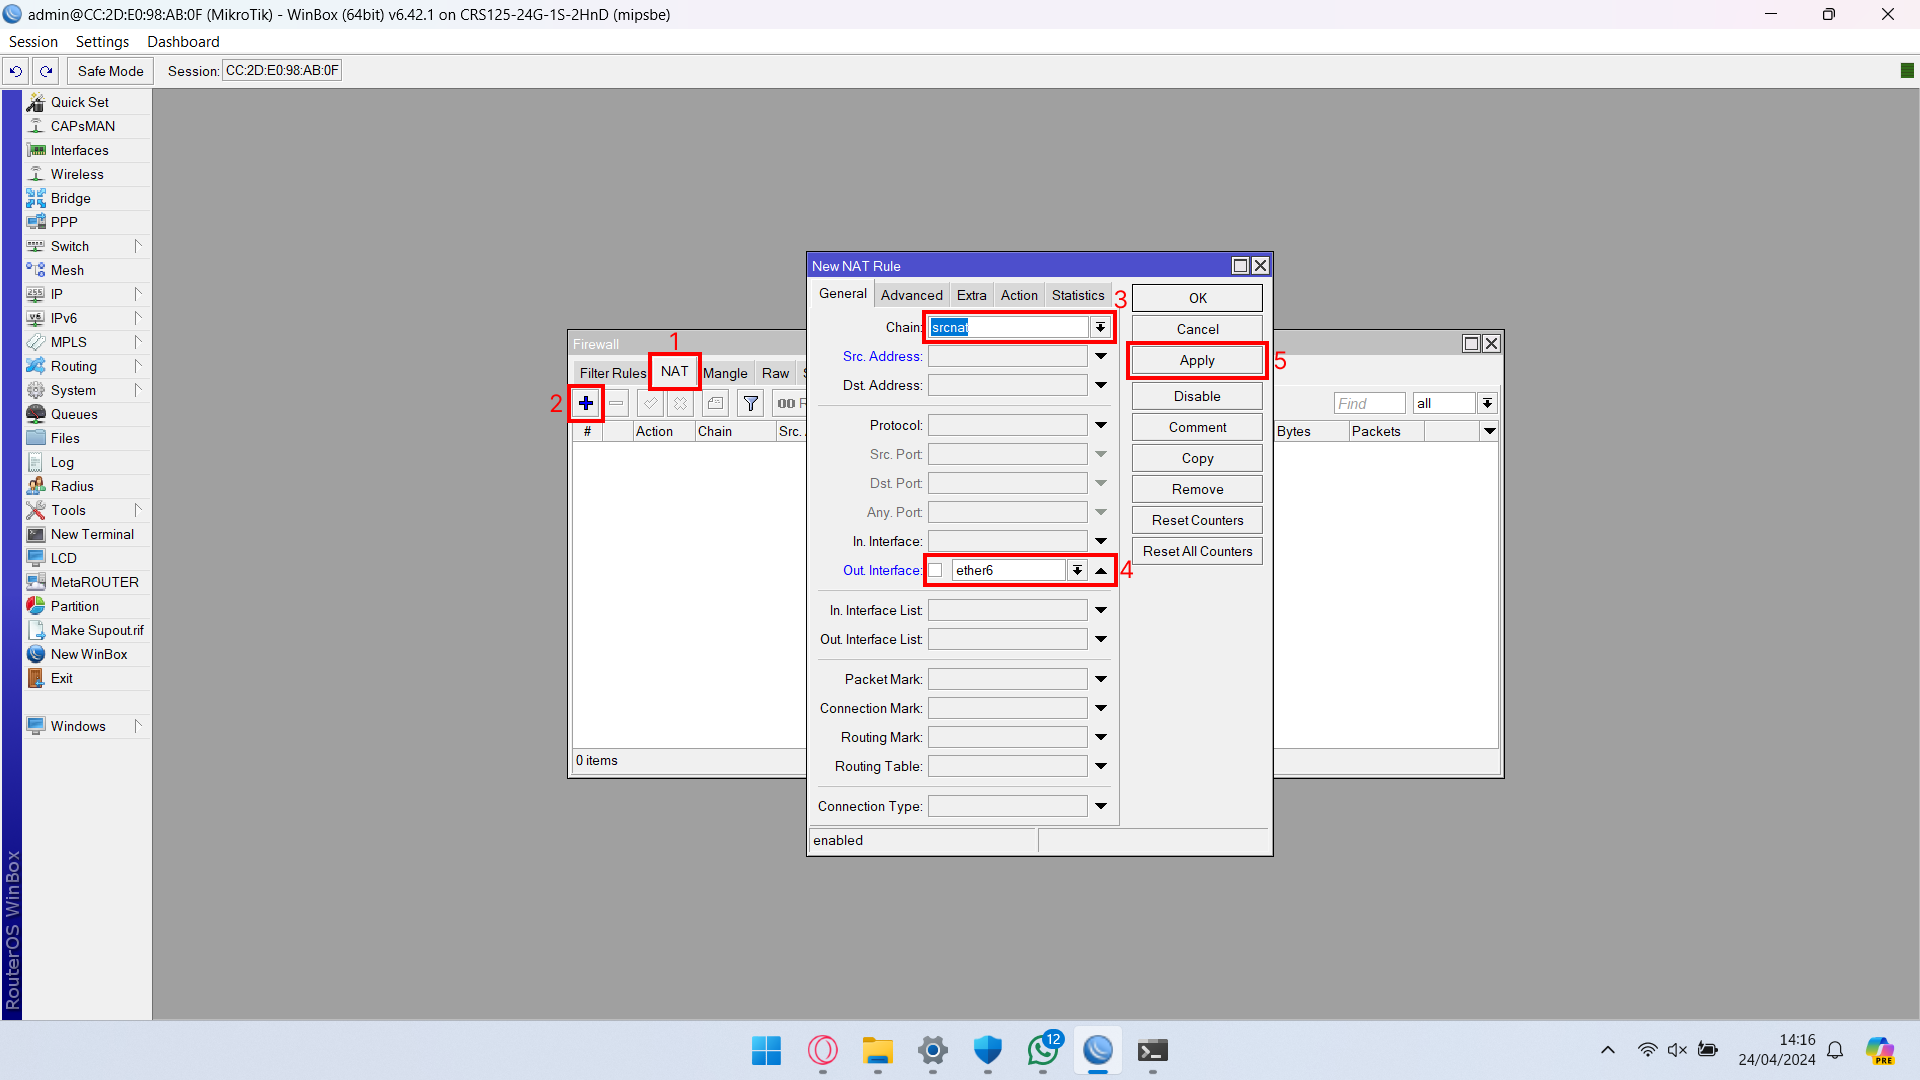
\includegraphics[width=0.5\linewidth]{P4/img/pc1/Step 15.png}
			\caption{Step 10.1}
			\label{fig:Step 10.1(PC 1)}
        \end{figure}
        \begin{figure}[H]
			\centering
			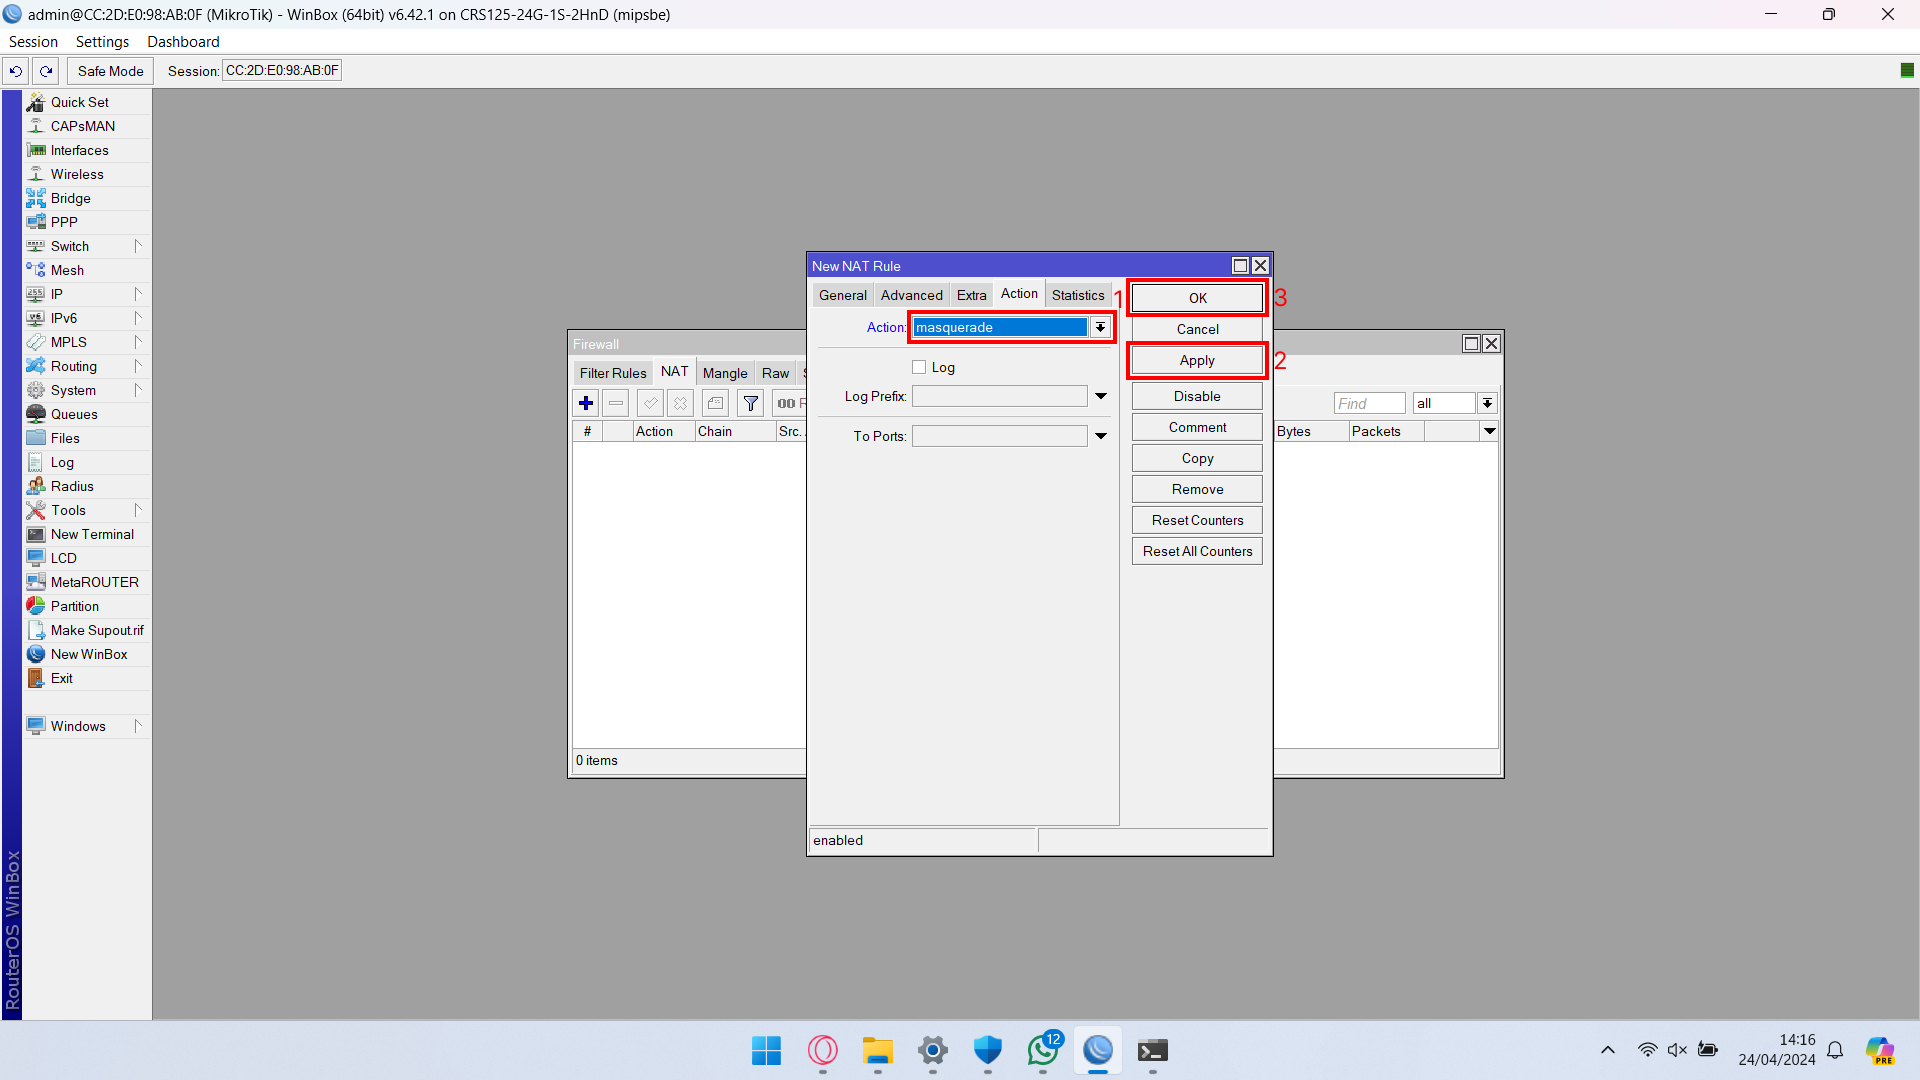
\includegraphics[width=0.8\linewidth]{P4/img/pc1/Step 14.png}
			\caption{Step 10.2}
			\label{fig:Step 10.2(PC 1)}
		\end{figure}	
    \end{enumerate}
	\textbf{Pengujian Konfigurasi}
	\begin{enumerate}
		\item Lakukan tes ping ke alamat Remote Address Router 2 untuk memastikan kedua Router sudah terhubung.
		\begin{figure}[H]
			\centering
			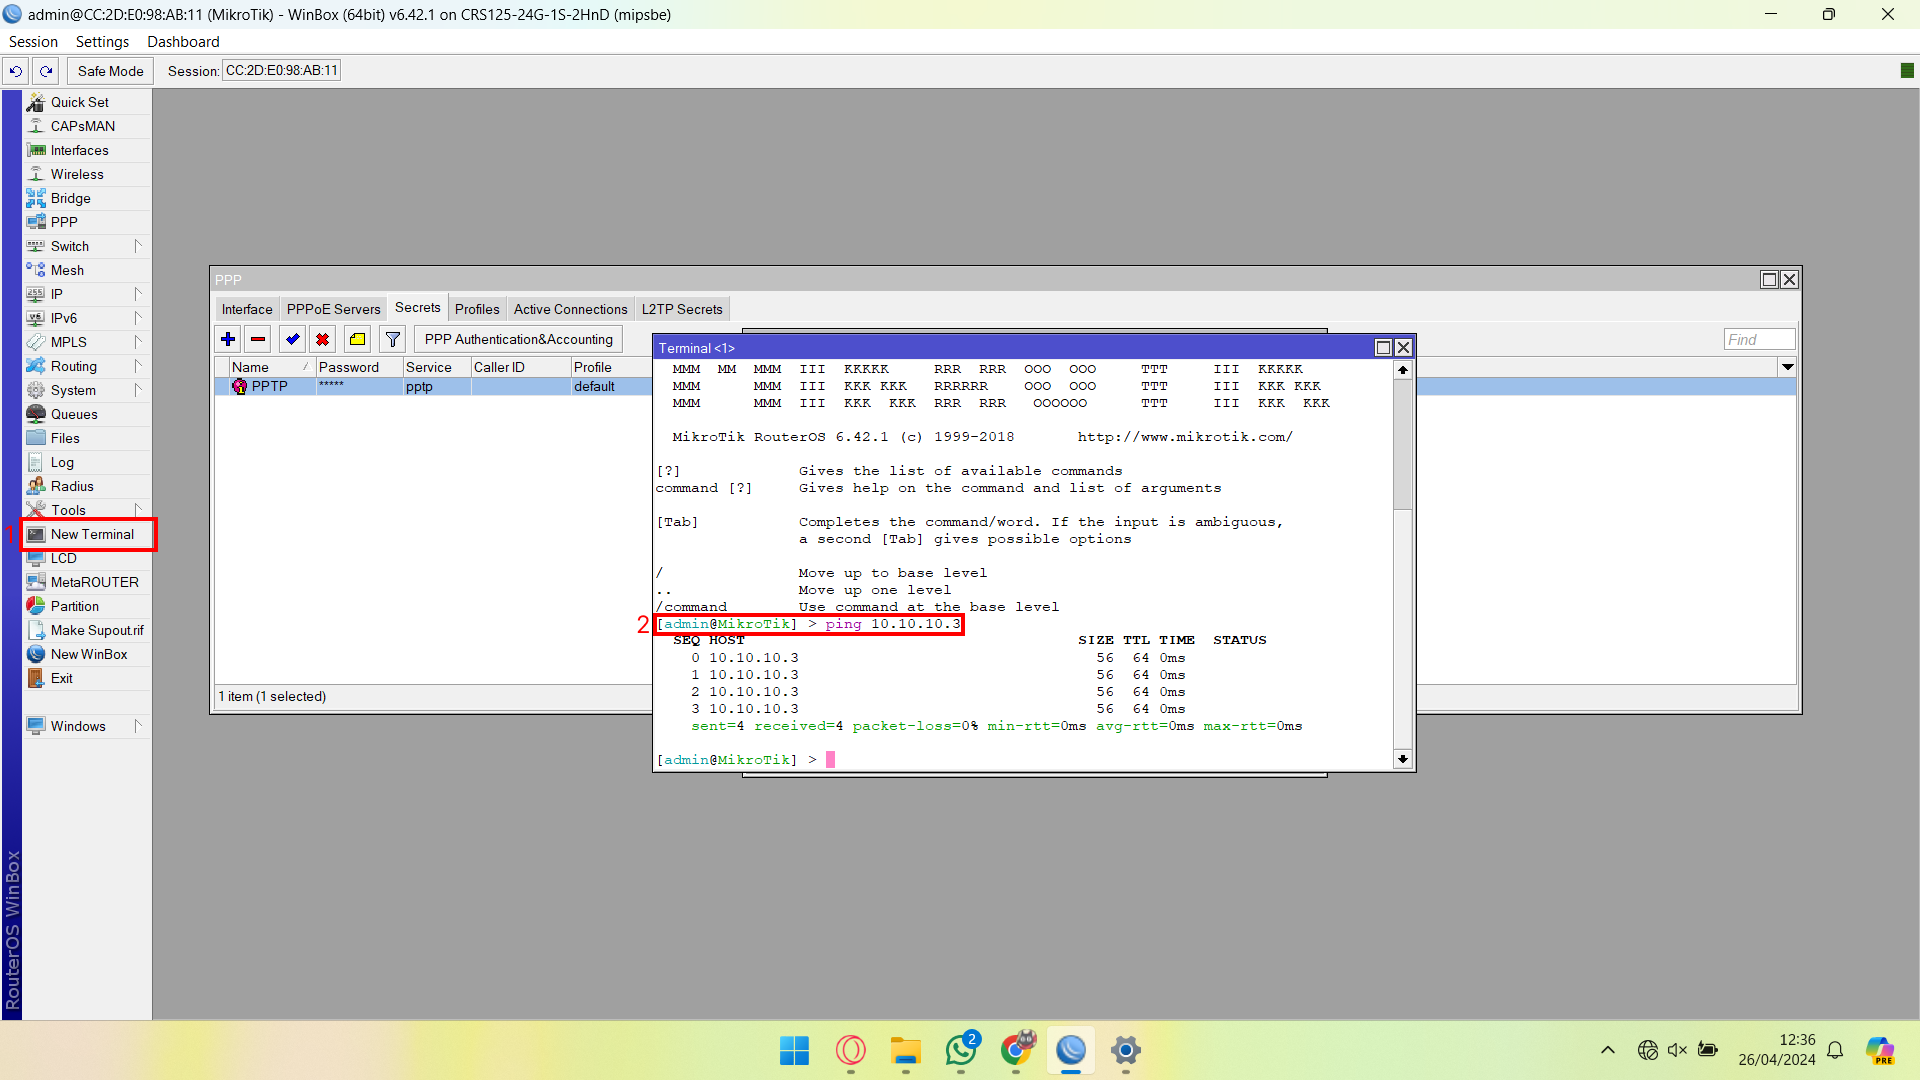
\includegraphics[width=0.8\linewidth]{P4/img/pc1/Step 9.png}
			\caption{Step 1}
			\label{fig:Ping Step 1(PC 1)}
		\end{figure}
		\item Lakukan tes ping ke PC 2 untuk memastikan kedua PC sudah terhubung.
		\begin{figure}[H]
			\centering
			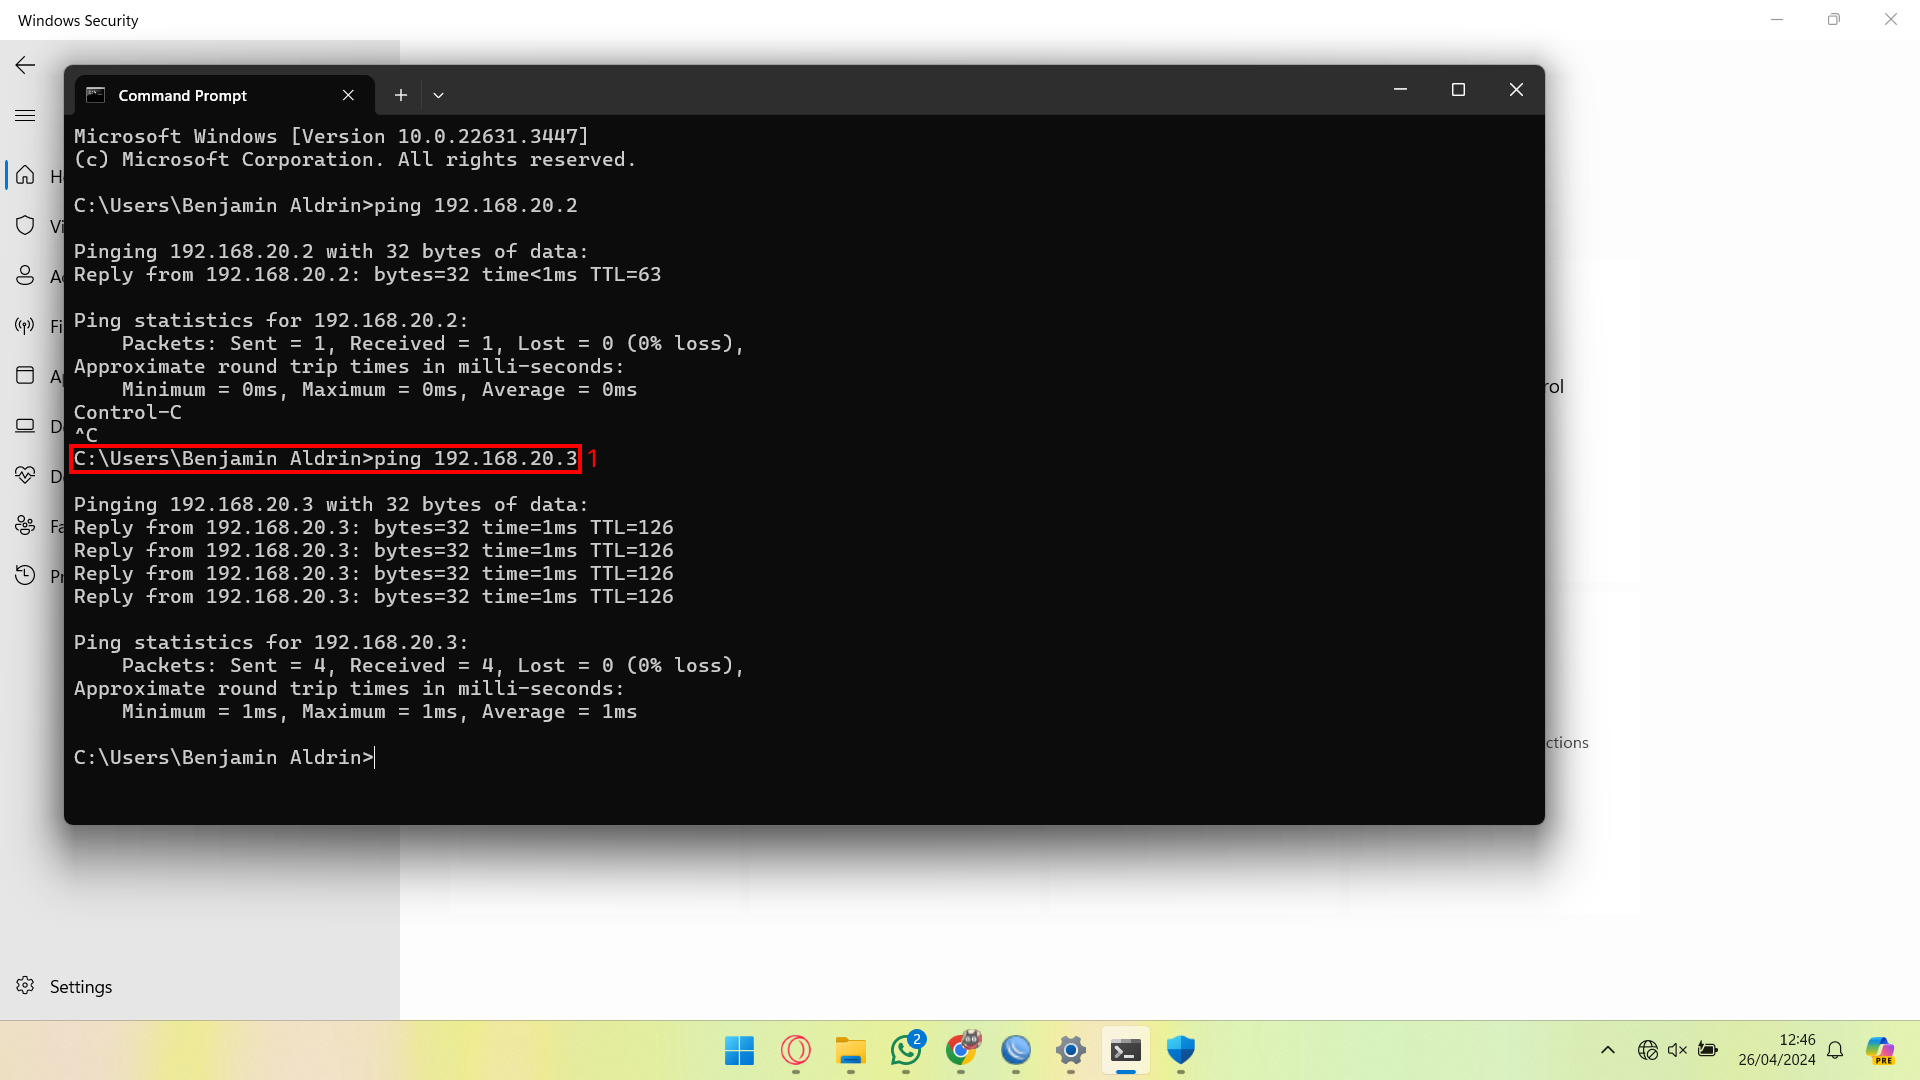
\includegraphics[width=0.8\linewidth]{P4/img/pc1/Step 10.png}
			\caption{Step 2}
			\label{fig:Ping Step 2(PC 1)}
		\end{figure}
	\end{enumerate}

    \textbf{Konfigurasi PC 2}
    \begin{enumerate}
        \item Hubungkan PC2 dengan Internet, bisa dilakukan menggunakan wifi ITS.
        \begin{figure}[H]
			\centering
			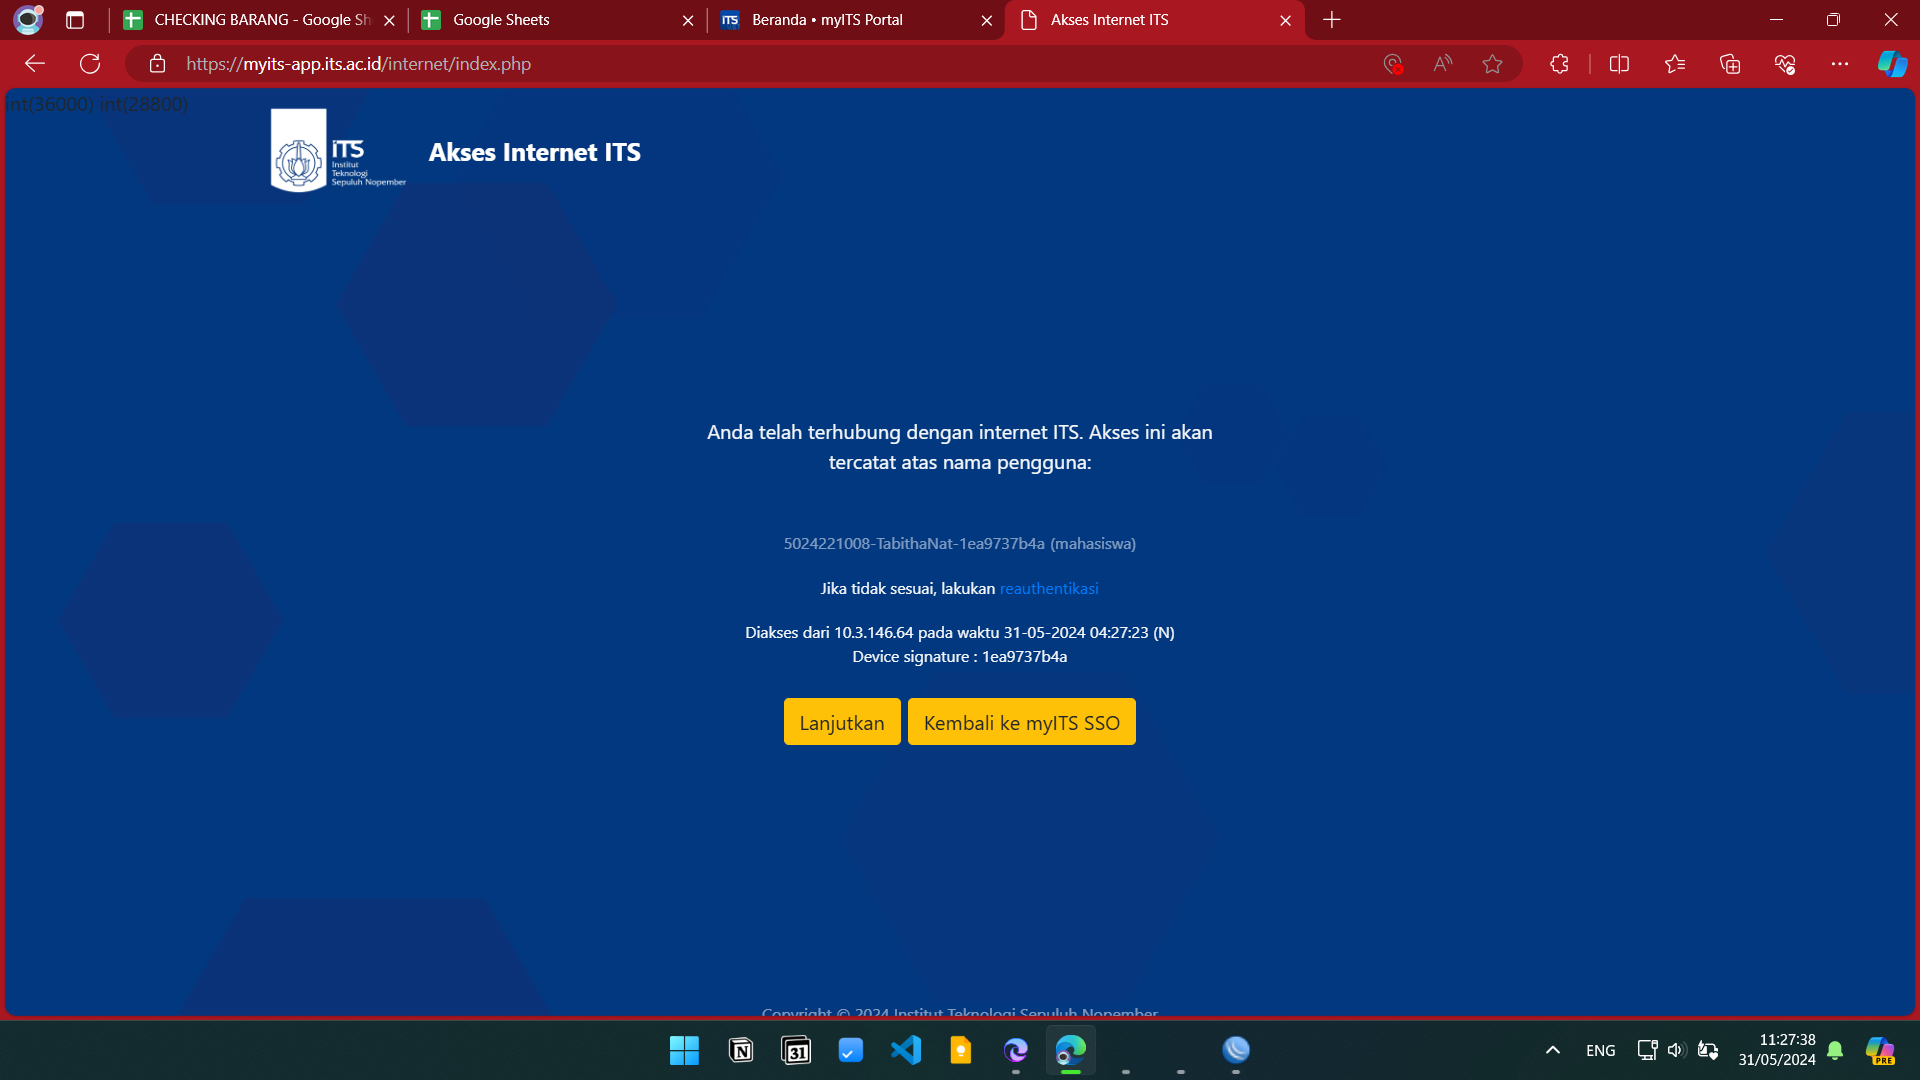
\includegraphics[width=0.5\linewidth]{P4/img/pc2/Step 1.png}
			\caption{Step 1}
			\label{fig:Step 1(PC 2)}
		\end{figure}
        \item Cek IP yang diterima PC2 dari ITS.
        \begin{figure}[H]
			\centering
			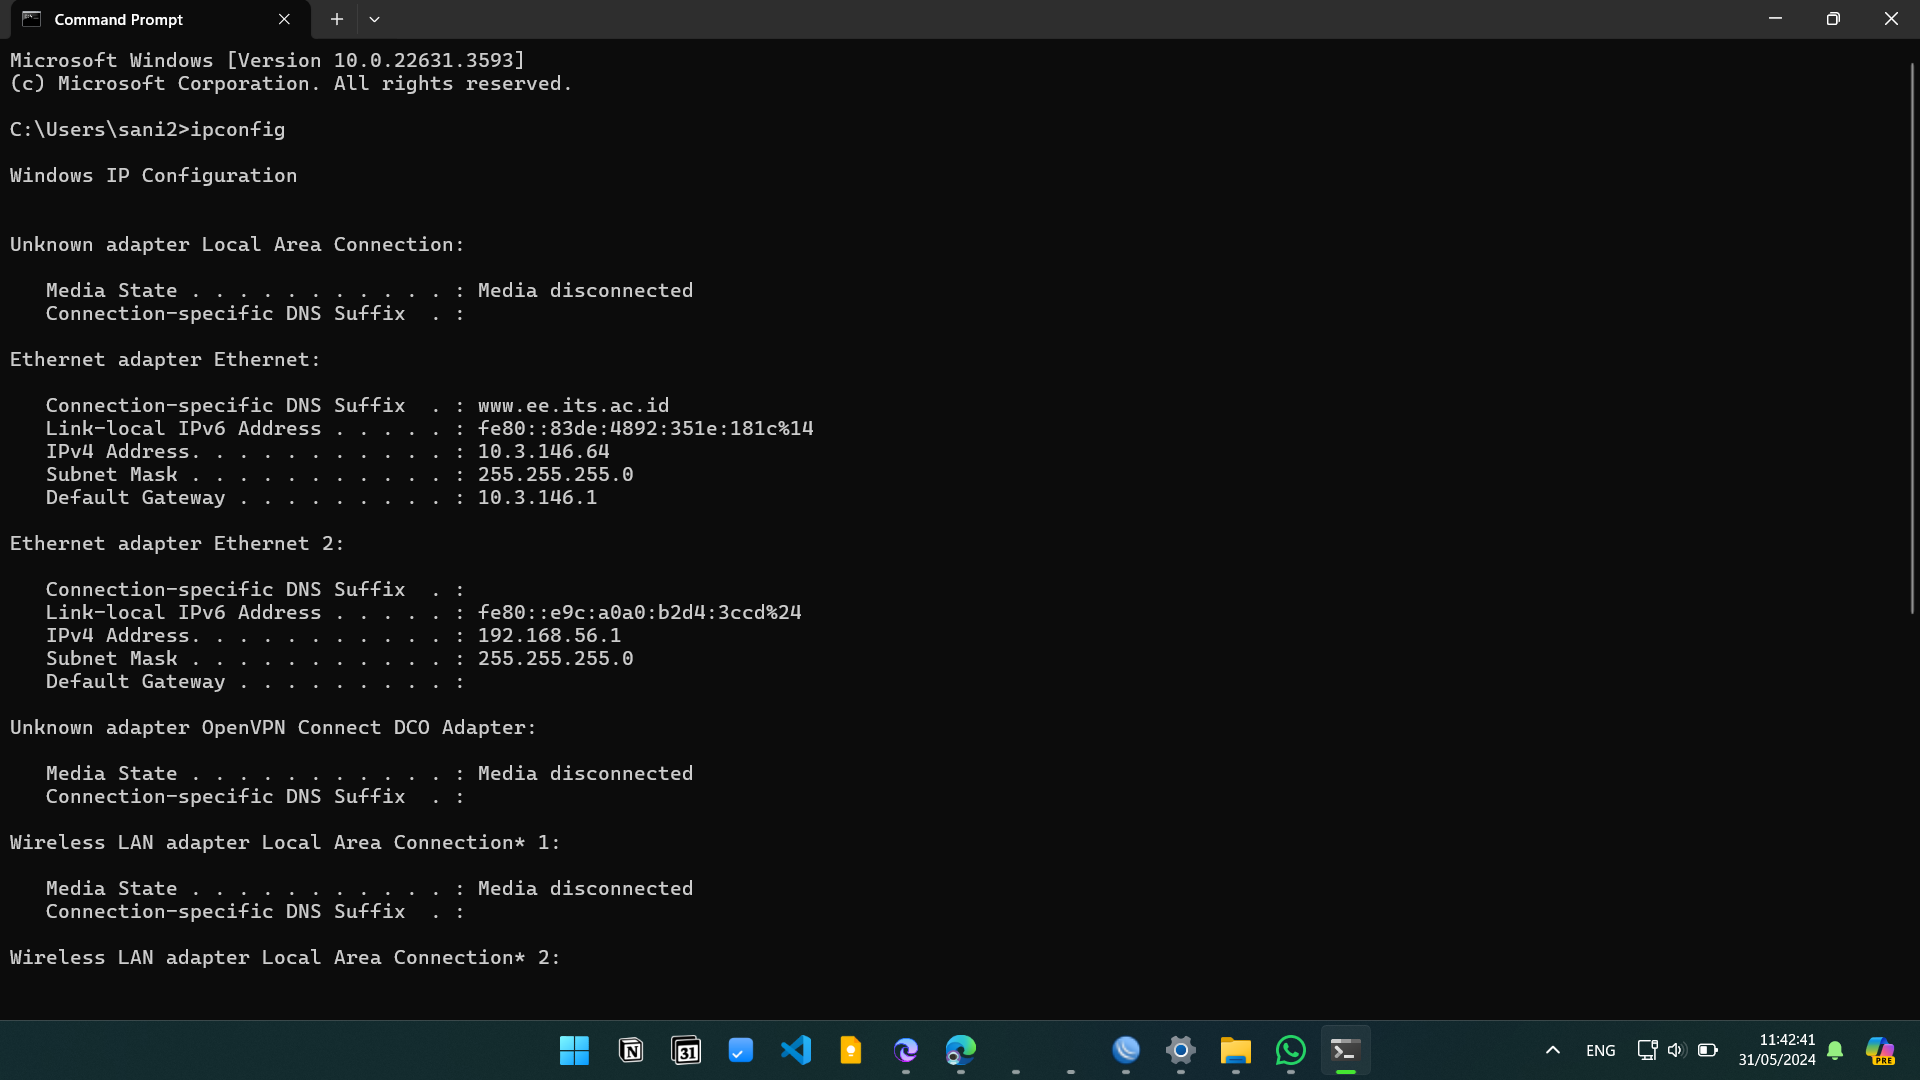
\includegraphics[width=0.5\linewidth]{P4/img/pc2/Step 2.png}
			\caption{Step 2}
			\label{fig:Step 2(PC 2)}
        \end{figure}
        \item Masuk ke dalam setting PC2 dan klik VPN.
        \begin{figure}[H]
			\centering
			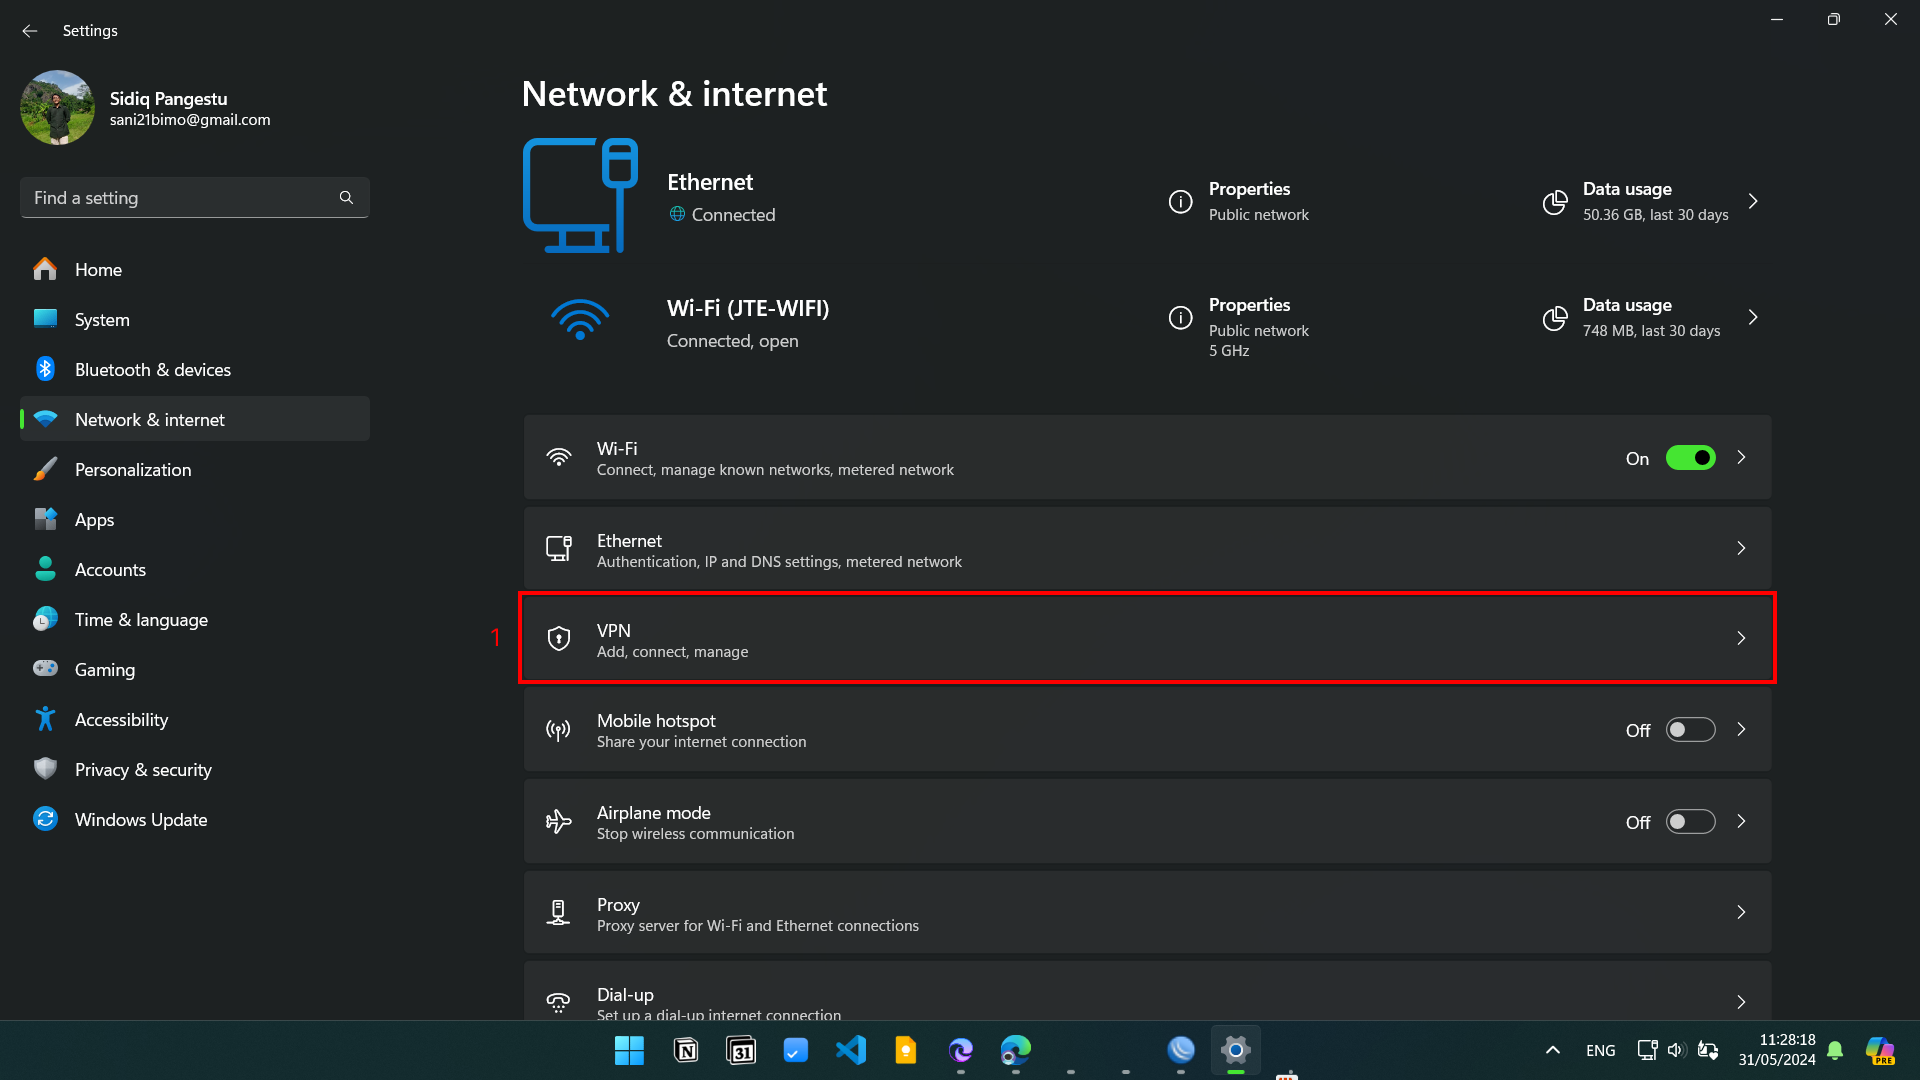
\includegraphics[width=0.8\linewidth]{P4/img/pc2/Step 3.png}
			\caption{Step 3}
			\label{fig:Step 3(PC 2)}
		\end{figure}
        \item Hubungkan client PPTP dengan server PPTP, untuk melakukan hal tersebut, buatlah koneksi VPN baru antara PC2 dengan Host Server. Pastikan menggunakan VPN type PPTP. Pastikan Username dan password sudah sesuai dengan konfigurasi Router1.
        \begin{figure}[H]
			\centering
			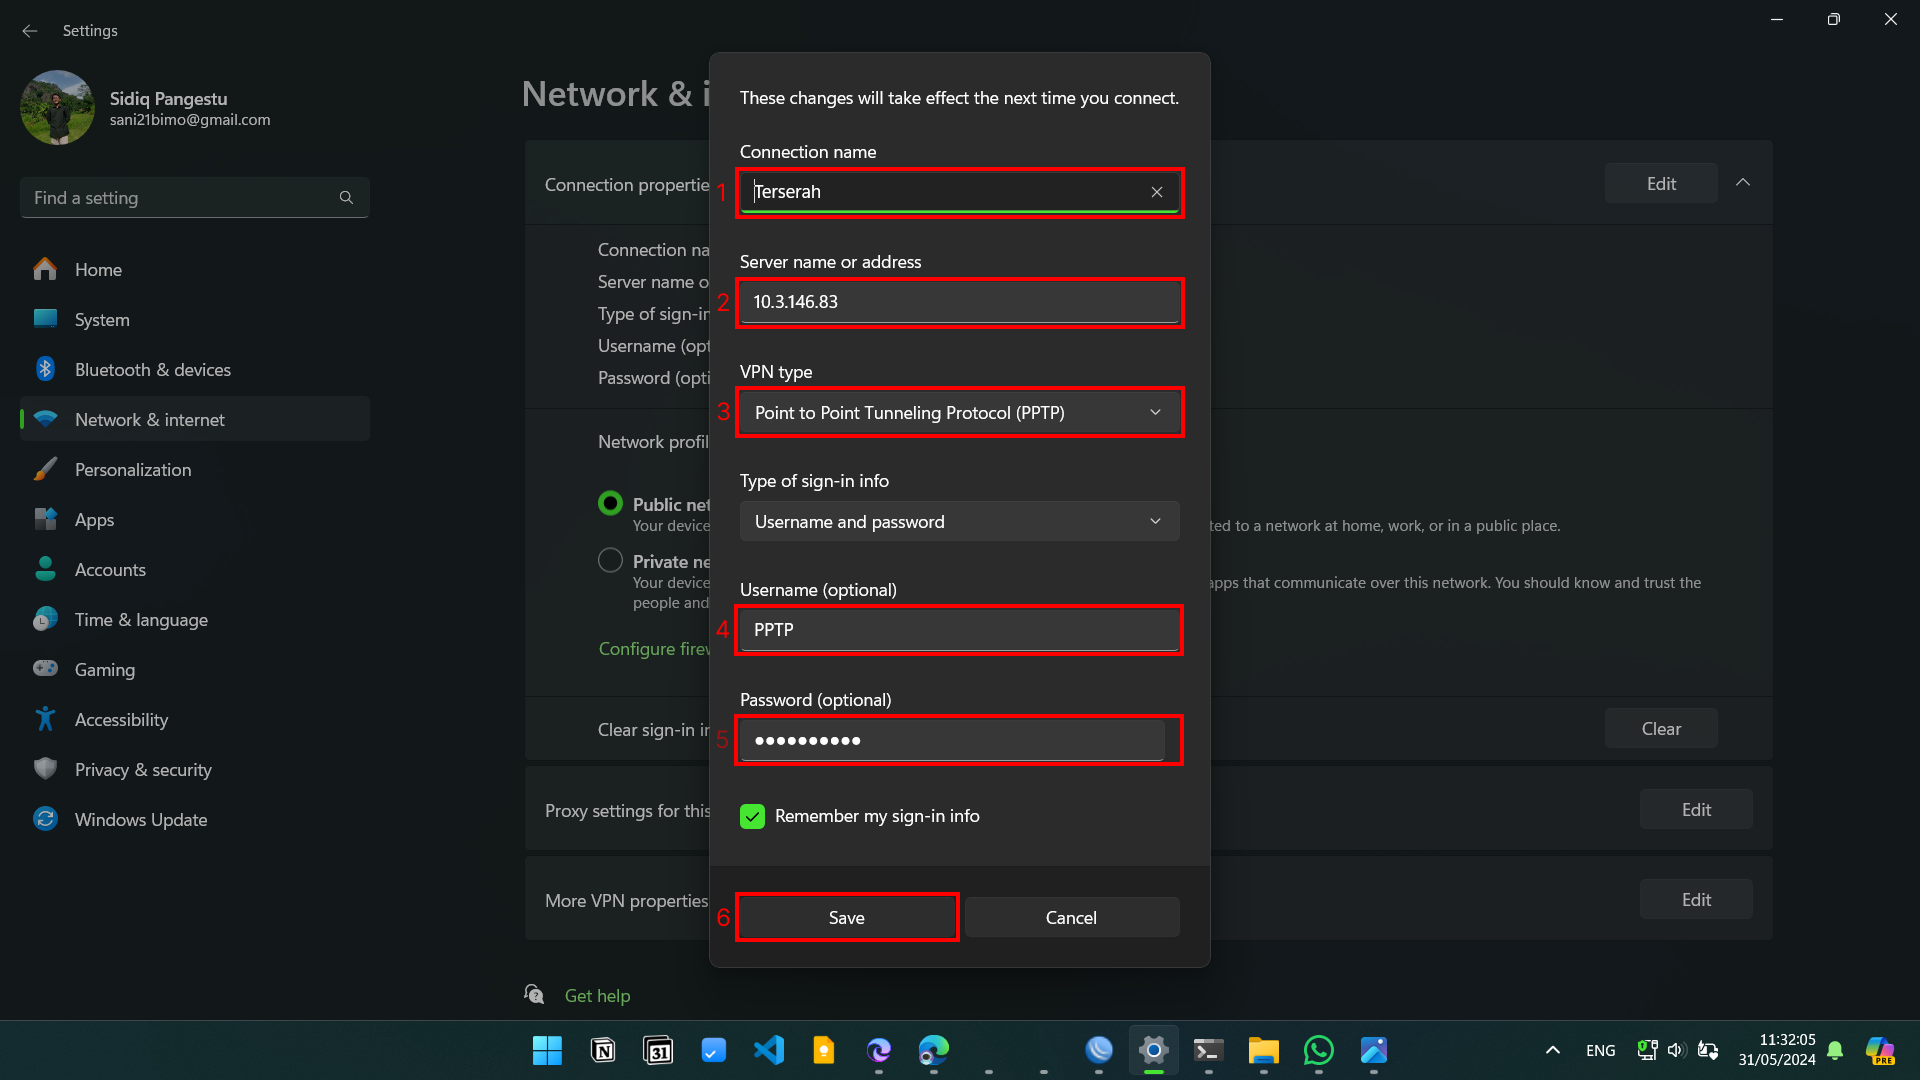
\includegraphics[width=0.8\linewidth]{P4/img/pc2/Step 4.png}
			\caption{Step 4}
			\label{fig:Step 4(PC 2)}
		\end{figure}
        \item Hubungkan ke VPN dengan cara klik tombol Connect
        \begin{figure}[H]
			\centering
			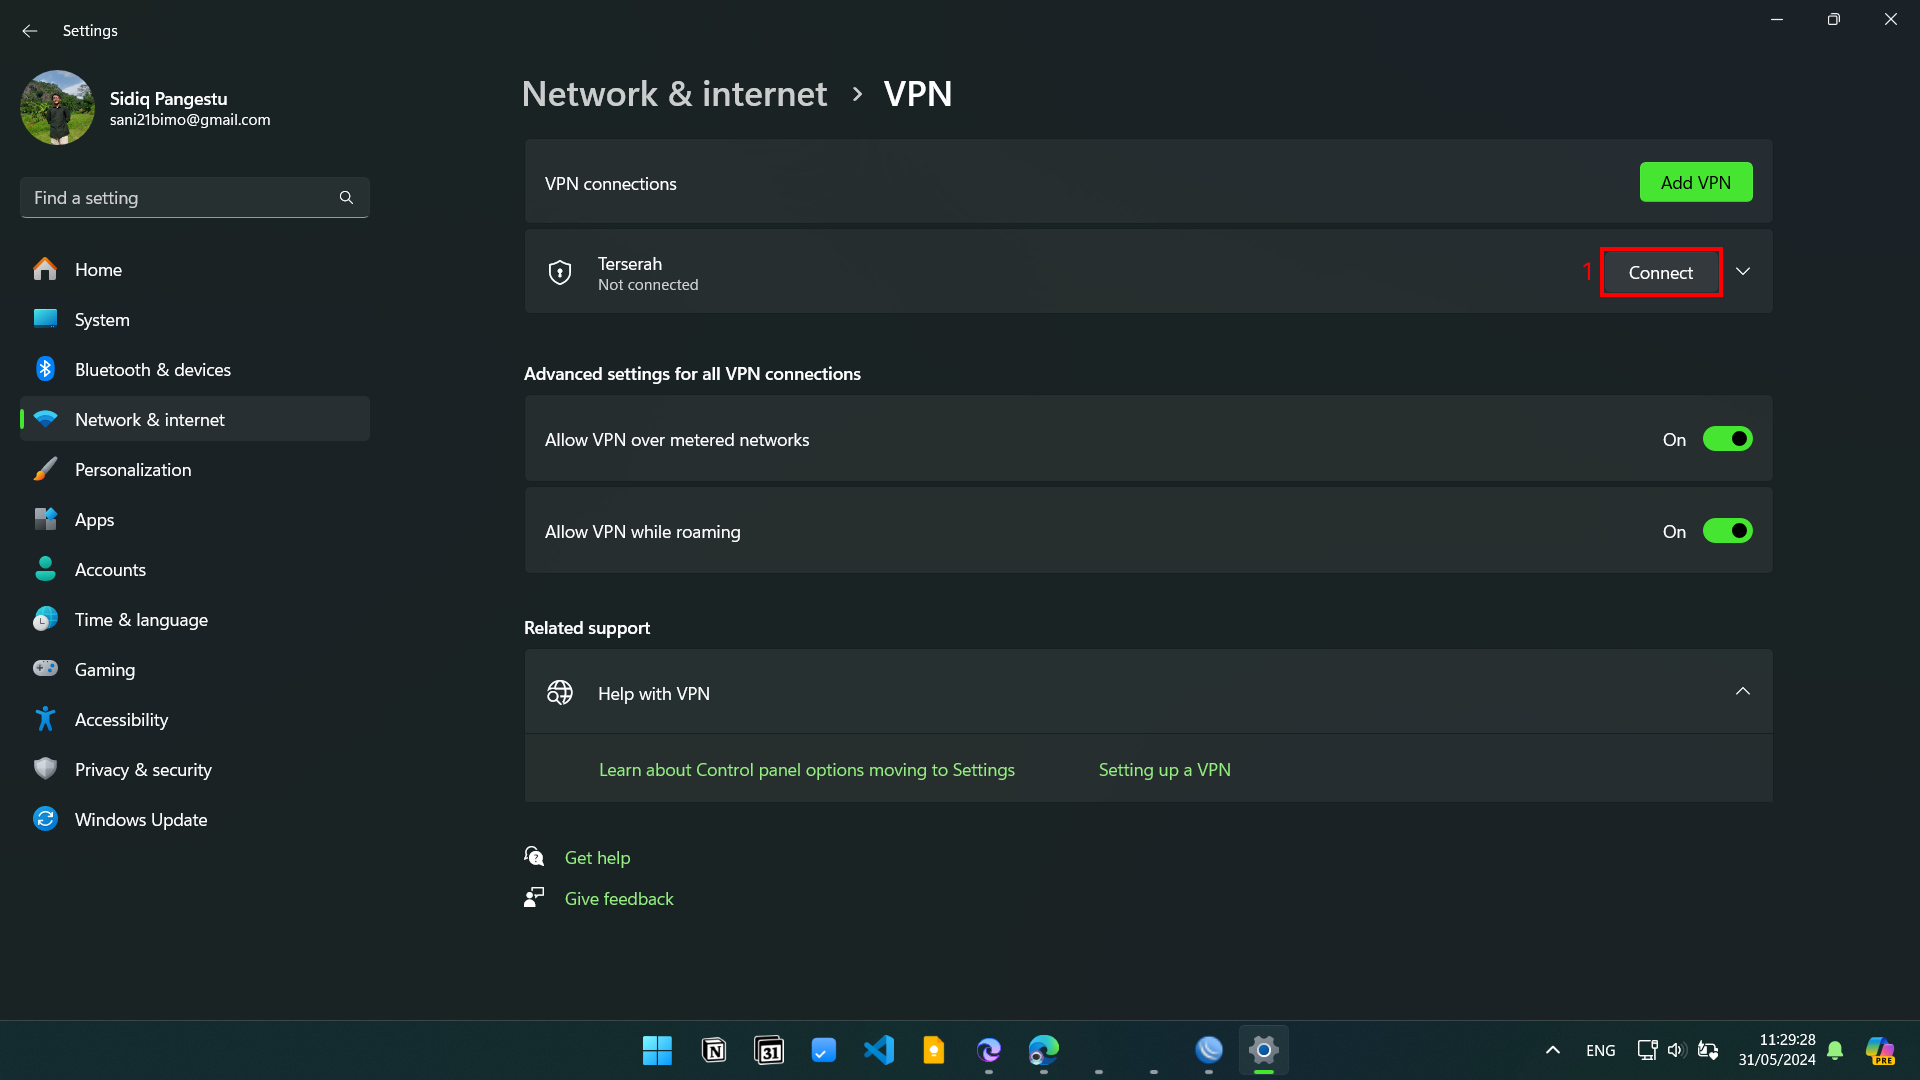
\includegraphics[width=0.8\linewidth]{P4/img/pc2/Step 5.png}
			\caption{Step 5}
			\label{fig:Step 5(PC 2)}
		\end{figure}
    \end{enumerate}

	\textbf{Pengujian Konfigurasi}
	\begin{enumerate}
		\item Lakukan tes ping ke alamat PC1 untuk memastikan VPN PPTP sudah terhubung.
		\begin{figure}[H]
			\centering
			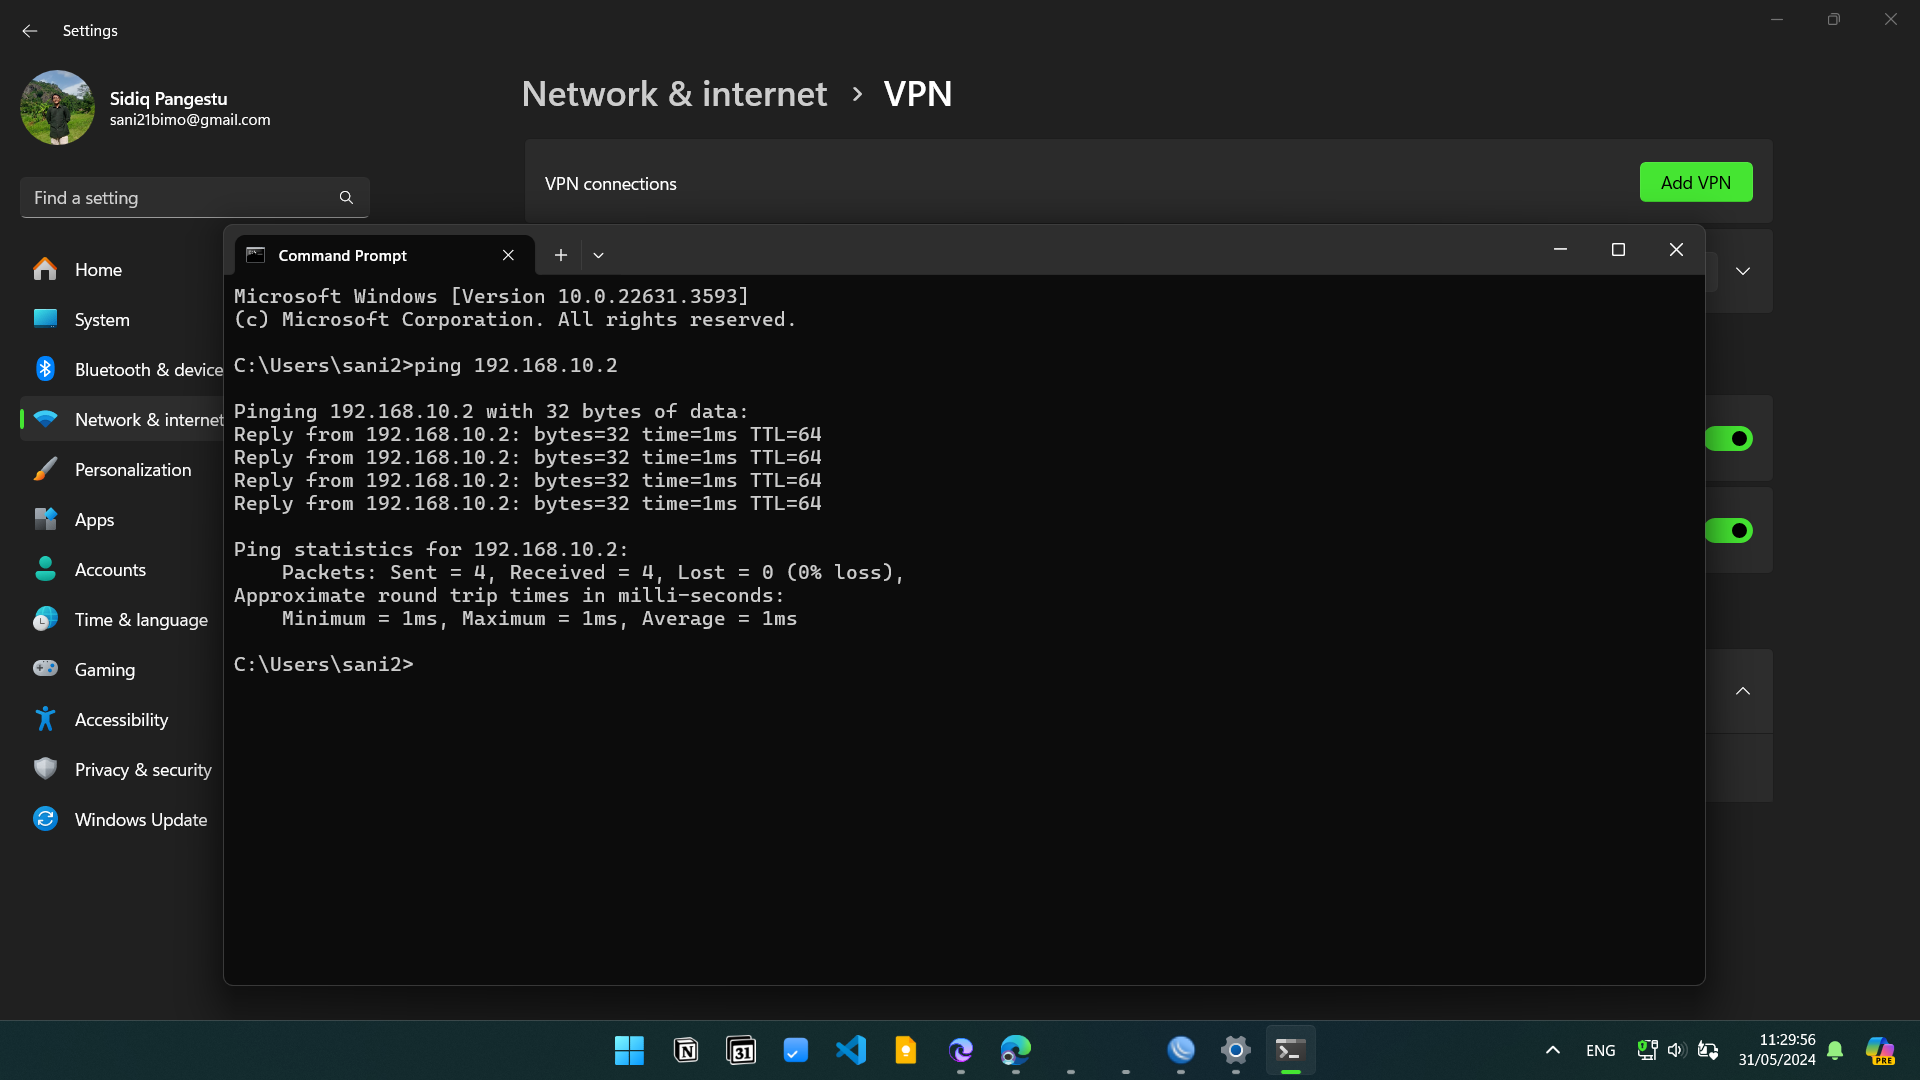
\includegraphics[width=0.8\linewidth]{P4/img/pc2/Step 6.png}
			\caption{Step 1}
			\label{fig:Ping Step 1(PC 2)}
		\end{figure}
	\end{enumerate}
\end{center}

%===========================================================%
\section{Hasil yang didapat}
Memahami penerapan dan penghubungan jaringan dengan menerapkan PPTP dengan VPN

%===========================================================%
\section{Kesimpulan}
Dalam mengkonfigurasi VPN, diperlukan pemahaman dasar mengenai metode PPTP, dan juga diperlukan ketelitian dan fokus agar berhasil
